% =====================================================================
%  Rapport — Projet Math en assurance et finance (ESPRIT, 5INFINI)
%  Diversification par apprentissage non supervisé sur la BVMT
%  Compilation : pdflatex (Overleaf par défaut) ou xelatex / lualatex.
%  Les figures sont dans figures/, les tableaux d'annexe dans annexes/.
% =====================================================================
\documentclass[11pt,a4paper]{article}

% ---------- langue et polices (pdflatex ou xelatex/lualatex) ----------
\usepackage{iftex}
\ifPDFTeX
  \usepackage[T1]{fontenc}
  \usepackage[utf8]{inputenc}
  \usepackage{lmodern}
  \usepackage[french]{babel}
\else
  \usepackage{fontspec}
  \usepackage{polyglossia}
  \setdefaultlanguage{french}
\fi

% ---------- mise en page ----------
\usepackage[a4paper,margin=2.5cm,headheight=14pt]{geometry}
\usepackage{microtype}
\usepackage{amsmath,amssymb}
\usepackage{graphicx}
\usepackage{booktabs,longtable,array,multirow,tabularx}
\usepackage{float}
\usepackage[font=small,labelfont=bf]{caption}
\usepackage{subcaption}
\usepackage{xcolor}
\usepackage{enumitem}
\usepackage{fancyhdr}
\usepackage{titlesec}
\usepackage[most]{tcolorbox}
\usepackage{csquotes}
\usepackage[hidelinks]{hyperref}

\definecolor{navy}{HTML}{1F3A5F}
\definecolor{orange}{HTML}{E07A1F}
\definecolor{fond}{HTML}{EEF2F7}

\titleformat{\section}{\Large\bfseries\color{navy}}{\thesection}{0.8em}{}
\titleformat{\subsection}{\large\bfseries\color{navy}}{\thesubsection}{0.8em}{}
\titleformat{\subsubsection}{\normalsize\bfseries\color{navy}}{\thesubsubsection}{0.8em}{}

\pagestyle{fancy}
\fancyhf{}
\fancyhead[L]{\small\color{navy}Diversification non supervisée sur la BVMT}
\fancyhead[R]{\small\color{navy}ESPRIT · 5INFINI}
\fancyfoot[C]{\small\thepage}
\renewcommand{\headrulewidth}{0.4pt}

\setlist{itemsep=2pt,topsep=4pt}
\setlength{\parskip}{4pt}
\graphicspath{{figures/}}

% encadré « à retenir »
\newtcolorbox{retenir}[1][À retenir]{colback=fond,colframe=navy,boxrule=0.6pt,arc=2mm,
  left=6pt,right=6pt,top=4pt,bottom=4pt,fonttitle=\bfseries,title=#1}
% marque visible pour ce que l'équipe doit compléter
\newcommand{\afaire}[1]{\textcolor{orange}{\textbf{[À compléter : #1]}}}
\newcommand{\pc}{~\%}

% =====================================================================
\begin{document}

% ---------------------------------------------------------------- garde
\begin{titlepage}
\centering
{\large ESPRIT School of Engineering\par}
{\normalsize Option Informatique financière · 5INFINI · Année universitaire 2026-2027\par}
\vspace{2.2cm}
{\color{navy}\rule{\linewidth}{1pt}\par\vspace{0.4cm}}
{\Huge\bfseries\color{navy} Diversifier par l'apprentissage\\[4pt] non supervisé à la Bourse de Tunis\par}
\vspace{0.4cm}
{\Large Critique de Rebai et al.\ (2021) et réplication\\ sur les données officielles de la BVMT, 2023-2026\par}
{\color{navy}\rule{\linewidth}{1pt}\par}
\vspace{1.2cm}
{\large Projet Math en assurance et finance\par}
\vspace{1.5cm}
{\large\bfseries Équipe\par}
\vspace{0.2cm}
{\large Nadhmi Rouissi · Youssef Mellouli · Safwen Haboubi\\ Chahine Saadellaoui · Haroun Chebaane · Ghassen Hamdi\par}
\vspace{1.2cm}
{\large Encadrant : \afaire{nom de l'encadrant}\par}
\vfill
{\large Novembre 2026\par}
\end{titlepage}

% ---------------------------------------------------------------- résumé
\section*{Résumé}
Rebai, Boukhris, Ncib et Ben Lasmar (2021) proposent de voir la diversification d'un portefeuille comme un problème de segmentation : regrouper les actions qui se ressemblent par k-means et repérer les actions anormales par Isolation Forest, sur la Bourse de Tunis avant et pendant le Covid-19. Nous analysons cet article, puis nous refaisons l'étude sur des données officielles récentes : 75 actions cotées à la Bourse des valeurs mobilières de Tunis (BVMT), du 02/01/2023 au 03/11/2026 (960 séances), après correction de 228 opérations sur titres.

Avec un taux sans risque de 7\pc{} (6,77\pc{} en taux continu), l'optimisation exacte de Markowitz donne un ratio de Sharpe maximal de 4,93, aussi peu réaliste que ceux de l'article : il est mesuré dans l'échantillon, sur un marché très haussier. La segmentation, dont le nombre de groupes est choisi par le vote de quatre critères, ne fait apparaître qu'une structure faible (silhouette inférieure à 0,5). Les groupes ne suivent pas les secteurs : ils séparent les titres liquides et liés au marché des titres volatils, peu échangés et peu liés au marché. La plupart des anomalies détectées par Isolation Forest sont des artefacts d'illiquidité, ce que l'article ne contrôlait pas. Retirer les deux features redondantes (kurtosis et VaR) ne change aucune de ces conclusions. La prochaine étape est de construire des portefeuilles à partir des groupes et de les tester hors échantillon.

\noindent\textbf{Mots-clés :} diversification, Markowitz, k-means, ACP, Isolation Forest, BVMT, liquidité, opérations sur titres.

\clearpage
\tableofcontents
\clearpage
\listoffigures
\listoftables
\clearpage

% =====================================================================
\section{Introduction}
% =====================================================================
\subsection{Contexte et objectif}
La diversification consiste à répartir son capital entre des actifs qui ne bougent pas tous ensemble, pour réduire le risque sans trop sacrifier le rendement. La réponse classique est l'optimisation de Markowitz (1952), qui demande d'estimer les rendements moyens et la matrice de covariance des actifs. L'article de référence propose une autre voie : utiliser l'apprentissage non supervisé pour regrouper les actions semblables, puis diversifier entre les groupes.

Notre projet a deux objectifs :
\begin{enumerate}
  \item \textbf{analyser et critiquer} l'article de Rebai et al.\ (2021) ;
  \item \textbf{refaire l'étude correctement} sur des données récentes et officielles de la BVMT, en vérifiant chaque choix de méthode, et préparer le test des portefeuilles construits à partir des groupes.
\end{enumerate}

\subsection{Organisation de l'équipe}
Le cahier des charges demande un responsable par rôle. Chaque membre reste responsable de la compréhension de l'ensemble du projet.

\begin{table}[H]\centering\small
\caption{Répartition des rôles}\label{tab:roles}
\begin{tabular}{lp{7.5cm}l}\toprule
Rôle & Responsabilités & Responsable \\ \midrule
Données & Collecte, nettoyage, opérations sur titres, rapport qualité & \afaire{nom} \\
Features et Markowitz & Indicateurs de risque, variance minimale, Sharpe maximal & \afaire{nom} \\
Segmentation & k-means, ACP, Isolation Forest, choix de $k$, interprétation & \afaire{nom} \\
Extension & Mise en œuvre de l'extension choisie & \afaire{nom} \\
Synthèse & Analyse critique, rapport \LaTeX{} et présentation & \afaire{nom} \\
\bottomrule\end{tabular}
\end{table}

\subsection{Plan du rapport}
La partie~I (sections~\ref{sec:art-objectif} à~\ref{sec:art-limites}) présente l'article et ses limites. La partie~II (sections~\ref{sec:notre-objectif} à~\ref{sec:interface}) présente notre travail : données, paramètres, Markowitz, segmentation, anomalies, contrôle de robustesse avec cinq features et interface de restitution. La section~\ref{sec:critique} discute les limites de notre propre travail, avant la conclusion. Les annexes donnent la déclaration d'usage de l'IA générative, la reproductibilité et les tableaux complets.

% =====================================================================
\part{L'article de référence}
% =====================================================================

\section{Objectif de l'article}\label{sec:art-objectif}
Rebai et al.\ (2021) étudient le marché boursier tunisien avant et pendant la crise du Covid-19. Leur idée est que la diversification peut se voir comme un problème de \textbf{segmentation} : si l'on sait regrouper les actions qui se ressemblent, il suffit de choisir des actions dans des groupes différents pour diversifier. Ils posent deux questions :
\begin{itemize}
  \item l'apprentissage non supervisé peut-il \textbf{regrouper} les actions qui se ressemblent ?
  \item peut-il \textbf{repérer les actions anormales}, potentiellement risquées ?
\end{itemize}
Les auteurs présentent cette approche comme une alternative, plus légère, à l'optimisation de portefeuille classique.

\section{Les données de l'article}\label{sec:art-donnees}
\begin{itemize}
  \item environ \textbf{85 sociétés} cotées, réparties en \textbf{12 secteurs} ;
  \item prix journaliers récupérés sur le site \textbf{investing.com} ;
  \item début en \textbf{mars 2019} et deux périodes : \textbf{avant le Covid} (310 séances) et \textbf{pendant} (de mars à décembre 2020) ;
  \item seul le \textbf{cours de clôture} est gardé, car les quatre prix du jour (ouverture, plus haut, plus bas, clôture) sont corrélés à 0,99 (Figure~7 de l'article).
\end{itemize}

\section{Les paramètres et leur calcul}\label{sec:art-features}
L'article part du rendement journalier simple (Équation~6 de l'article) :
\begin{equation}
R_t = \frac{P_t - P_{t-1}}{P_{t-1}}.
\end{equation}
Chaque action est ensuite décrite par sept \emph{features} :
\begin{itemize}
  \item le \textbf{rendement} moyen ;
  \item la \textbf{volatilité}, qui mesure la dispersion des rendements ;
  \item le \textbf{skewness}, qui mesure l'asymétrie de leur distribution ;
  \item le \textbf{kurtosis}, qui mesure l'épaisseur des queues, donc la fréquence des valeurs extrêmes ;
  \item la \textbf{VaR} à 95\pc{}, la perte d'un des 5\pc{} pires jours ;
  \item la \textbf{CVaR} à 95\pc{}, la perte moyenne sur ces pires jours ;
  \item le \textbf{bêta}, la sensibilité de l'action au marché.
\end{itemize}
Chaque action devient ainsi un point dans un espace à sept dimensions.

\section{Markowitz dans l'article}\label{sec:art-markowitz}
Les auteurs construisent une frontière efficiente en \textbf{simulant 100\,000 portefeuilles au hasard} (Figures~1 à~4 de l'article). Le tableau~\ref{tab:art-markowitz} résume leurs résultats.

\begin{table}[H]\centering\small
\caption{Portefeuilles de Markowitz publiés dans l'article}\label{tab:art-markowitz}
\begin{tabular}{lcc}\toprule
 & Avant le Covid & Pendant le Covid \\ \midrule
Sharpe maximal & \textbf{4,01} (rendement 39,9\pc{}, volatilité 10,0\pc{}) & \textbf{4,86} (rendement 90,1\pc{}, volatilité 18,5\pc{}) \\
Variance minimale & rendement 32,0\pc{}, volatilité 8,3\pc{} & rendement 37,3\pc{}, volatilité 11,8\pc{} \\
\bottomrule\end{tabular}
\end{table}
Des ratios de Sharpe de 4 à 5 sont exceptionnellement élevés pour un marché réel ; nous y revenons dans les limites (section~\ref{sec:art-limites}).

\section{Segmentation et anomalies : la méthode de l'article}\label{sec:art-methode}
\begin{enumerate}
  \item \textbf{K-means} avec $k = 7$ groupes, choisi à l'aide de la silhouette, de l'indice de Calinski-Harabasz et de la méthode du coude (Figures~11 à~13 de l'article).
  \item Deux espaces de travail : le plan \textbf{rendement-volatilité} seul, ou \textbf{toutes les features après ACP}, les composantes retenues expliquant 51 à 55\pc{} de la variance.
  \item \textbf{Isolation Forest} avec un taux de contamination de 5\pc{} pour repérer les actions atypiques.
\end{enumerate}
K-means forme des groupes ; Isolation Forest repère les cas qui ne ressemblent à aucun autre.

\section{Ce que l'article a trouvé}\label{sec:art-resultats}
\begin{itemize}
  \item Dans le plan rendement-volatilité, les actions dessinent une \textbf{forme en triangle} (Figure~15 de l'article). Les banques tombent dans un même groupe, sauf UBCI.
  \item \textbf{Anomalies} : MIP, STEQ, ELBEN, SITX et AST avant le Covid ; SIMP, STEQ, ALKM, SITX et TINV pendant.
  \item \textbf{Vérification dans la presse} (ilboursa) : STEQ a été radiée (janvier 2021), AMS radiée (avril 2021) et UADH suspendue (mars 2021).
\end{itemize}
Plusieurs titres signalés ont donc ensuite connu de vrais problèmes, et les auteurs en concluent que la méthode fonctionne.

\section{Les limites de l'article}\label{sec:art-limites}
\subsection{Ce que la preuve ne montre pas}
\begin{enumerate}
  \item \textbf{Aucun portefeuille n'est construit à partir des clusters}, et il n'y a \textbf{pas de test hors échantillon}. L'idée de départ, diversifier entre les groupes, n'est donc jamais testée.
  \item \textbf{Les features décrivent chaque action seule}, pas la façon dont les actions bougent ensemble. Or la diversification dépend justement des co-mouvements, c'est-à-dire de la covariance, que k-means sur des features individuelles n'utilise pas.
  \item \textbf{Des chiffres peu réalistes} : rendements de 31 à 90\pc{} et Sharpe de 3 à 5. Le Sharpe y vaut rendement divisé par volatilité : le taux sans risque est donc implicitement nul, sans que ce soit dit, alors que le taux du marché monétaire tunisien était de l'ordre de 7\pc{}.
  \item \textbf{Le choix $k = 7$ est fragile} : dans l'article lui-même, la silhouette est plus haute à $k = 2$.
  \item \textbf{L'étude n'est pas reproductible} : données sans date d'extraction, sans code, prises sur un site non officiel.
\end{enumerate}

\subsection{Points demandés par le cahier des charges}
\paragraph{L'argument de complexité.} L'article justifie l'apprentissage non supervisé par un coût de calcul plus faible que celui de Markowitz (k-means de l'ordre de $O(n^2)$, inversion de la covariance en $O(n^3)$). Pour $n = 85$ actifs, inverser une matrice $85 \times 85$ demande environ $6 \times 10^5$ opérations, soit quelques millisecondes : ce n'est pas un obstacle. Le vrai coût vient de la \textbf{simulation de 100\,000 portefeuilles}, chacun demandant un produit $w^\top \Sigma w$ en $O(n^2)$, soit environ $7 \times 10^8$ opérations. Une optimisation quadratique exacte, comme la nôtre, évite cette simulation et donne une solution meilleure.

\paragraph{CAPM et théorie de Markowitz.} Il faut distinguer deux cadres. La théorie de Markowitz est un problème d'\emph{optimisation} : choisir des poids qui minimisent la variance pour un rendement donné, à partir de $\mu$ et $\Sigma$. Le CAPM est un modèle d'\emph{équilibre} : il relie le rendement attendu d'un titre à son bêta et au taux sans risque. Le bêta, utilisé comme feature, vient du CAPM ; le ratio de Sharpe et la droite de marché des capitaux supposent un taux sans risque explicite, que l'article ne donne pas.

\paragraph{La cohérence des périodes.} Les deux périodes n'ont pas la même longueur (310 séances avant le Covid, environ neuf mois pendant). Les estimations de rendement, de volatilité et surtout de VaR et de kurtosis sur quelques mois sont très bruitées, et la comparaison entre les deux périodes en est fragilisée.

\begin{retenir}
L'article a une bonne idée, mais une preuve incomplète : il ne teste pas les portefeuilles, ne mesure pas la qualité de ses groupes et ne contrôle pas la liquidité des titres qu'il qualifie d'anormaux.
\end{retenir}

% =====================================================================
\part{Notre travail : la BVMT de 2023 à 2026}
% =====================================================================

\section{Notre objectif et notre démarche}\label{sec:notre-objectif}
Nous gardons la même question, mais avec les sociétés cotées aujourd'hui et des données récentes. À terme, les groupes doivent mener à des portefeuilles, comparés au portefeuille équipondéré (1/N) et à Markowitz. Nous gardons l'idée de l'article et nous corrigeons le protocole :
\begin{itemize}
  \item données officielles, datées et reproductibles ;
  \item prix corrigés des opérations sur titres avant tout calcul ;
  \item optimisation exacte au lieu d'une simulation ;
  \item choix du nombre de groupes par plusieurs critères, avec alertes explicites ;
  \item vérification de la nature de chaque anomalie, en particulier de la liquidité ;
  \item chaque résultat refait sur les seuls titres liquides.
\end{itemize}
Le travail suit les étapes du cahier des charges : données (S2), features et Markowitz (S3), segmentation et anomalies (S4), complétées par un contrôle de robustesse à cinq features (S4b).

\section{Nos données}\label{sec:donnees}
\subsection{Sources et période}
Toutes les données viennent de \textbf{sources officielles de la Bourse de Tunis} :
\begin{itemize}
  \item les \textbf{archives annuelles} de cotation et d'indices de 2023 à 2025 ;
  \item les \textbf{bulletins officiels quotidiens} pour 2026 (209 bulletins PDF, dont la liste exacte est conservée dans le dépôt).
\end{itemize}
La période va du \textbf{02/01/2023 au 03/11/2026}, soit \textbf{960 séances} et 959 rendements journaliers, sans valeur manquante. Les données ont été extraites le 04/11/2026.

\subsection{Univers de titres}
Les sources contiennent 85 sociétés. Dix ne sont plus cotées au 03/11/2026 (par exemple AMS, SITEX ou la Société tunisienne du sucre) et sont retirées : il reste \textbf{75 titres}. Un titre est dit \textbf{liquide} s'il est échangé au moins 60\pc{} des séances : 57 titres sont liquides et 18 peu liquides (figure~\ref{fig:liquidite}).

\begin{figure}[H]\centering
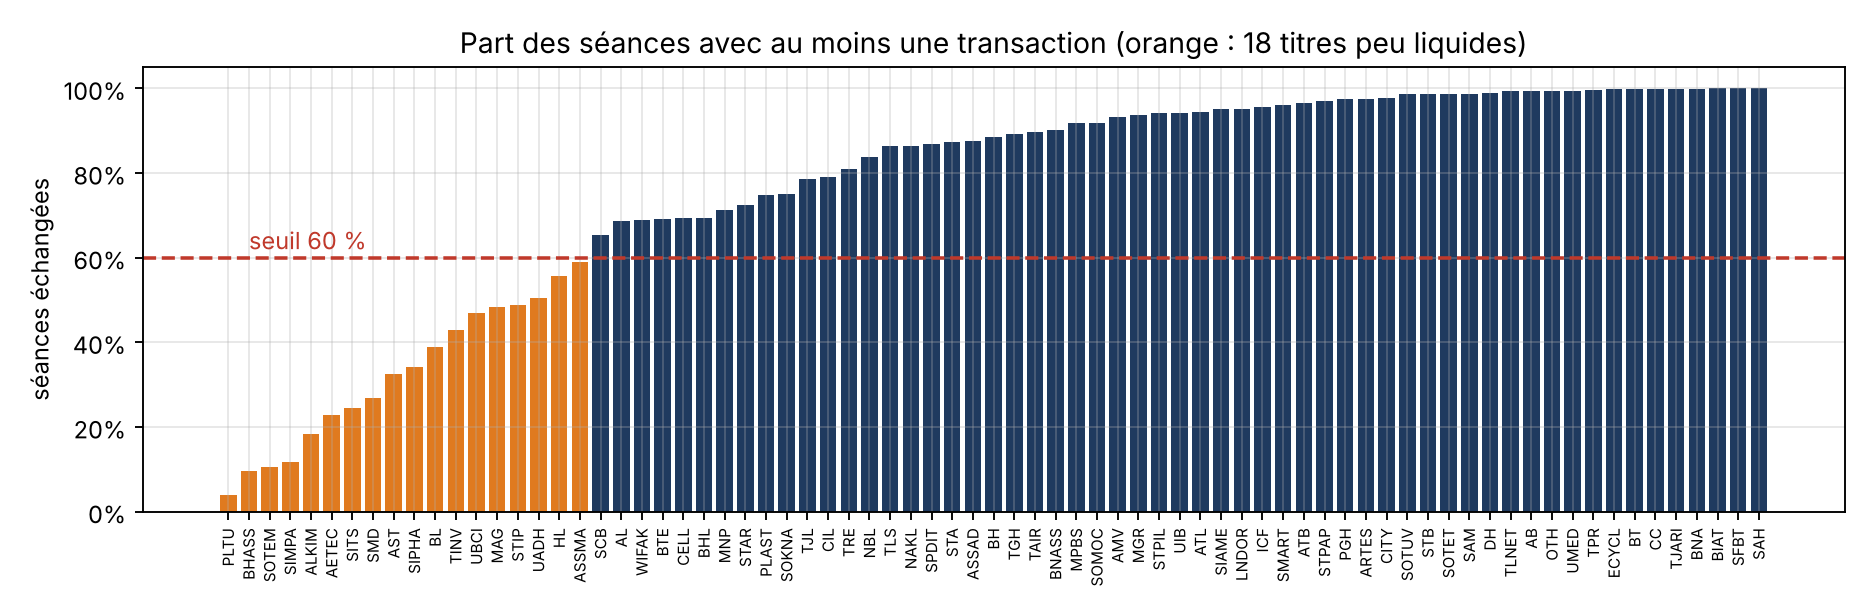
\includegraphics[width=\linewidth]{liquidite_75_titres.png}
\caption{Part des séances échangées pour les 75 titres. Un titre peu liquide a beaucoup de jours sans transaction : son prix ne bouge pas et ses rendements sont nuls.}\label{fig:liquidite}
\end{figure}

La liquidité jouera un rôle central dans la suite : un titre presque jamais échangé a une volatilité calculée très faible, non parce qu'il est peu risqué, mais parce que son prix ne bouge pas.

\subsection{Correction des opérations sur titres}
Les dividendes, attributions gratuites et divisions d'actions font baisser mécaniquement le cours sans perte pour l'actionnaire. Sans correction, ces baisses apparaissent comme de faux rendements négatifs. La BVMT publie chaque jour un \textbf{cours de référence}, qui tient compte de ces opérations. Nous détectons une opération quand le cours de référence diffère de la clôture de la veille, avec le facteur
\begin{equation}
f_t = \frac{\text{référence}_t}{\text{clôture}_{t-1}},
\end{equation}
et nous calculons le rendement du jour à partir du cours de référence (section~\ref{sec:features}). Nous trouvons ainsi \textbf{228 opérations sur titres} (détail en annexe~\ref{ann:ost}).

\begin{figure}[H]\centering
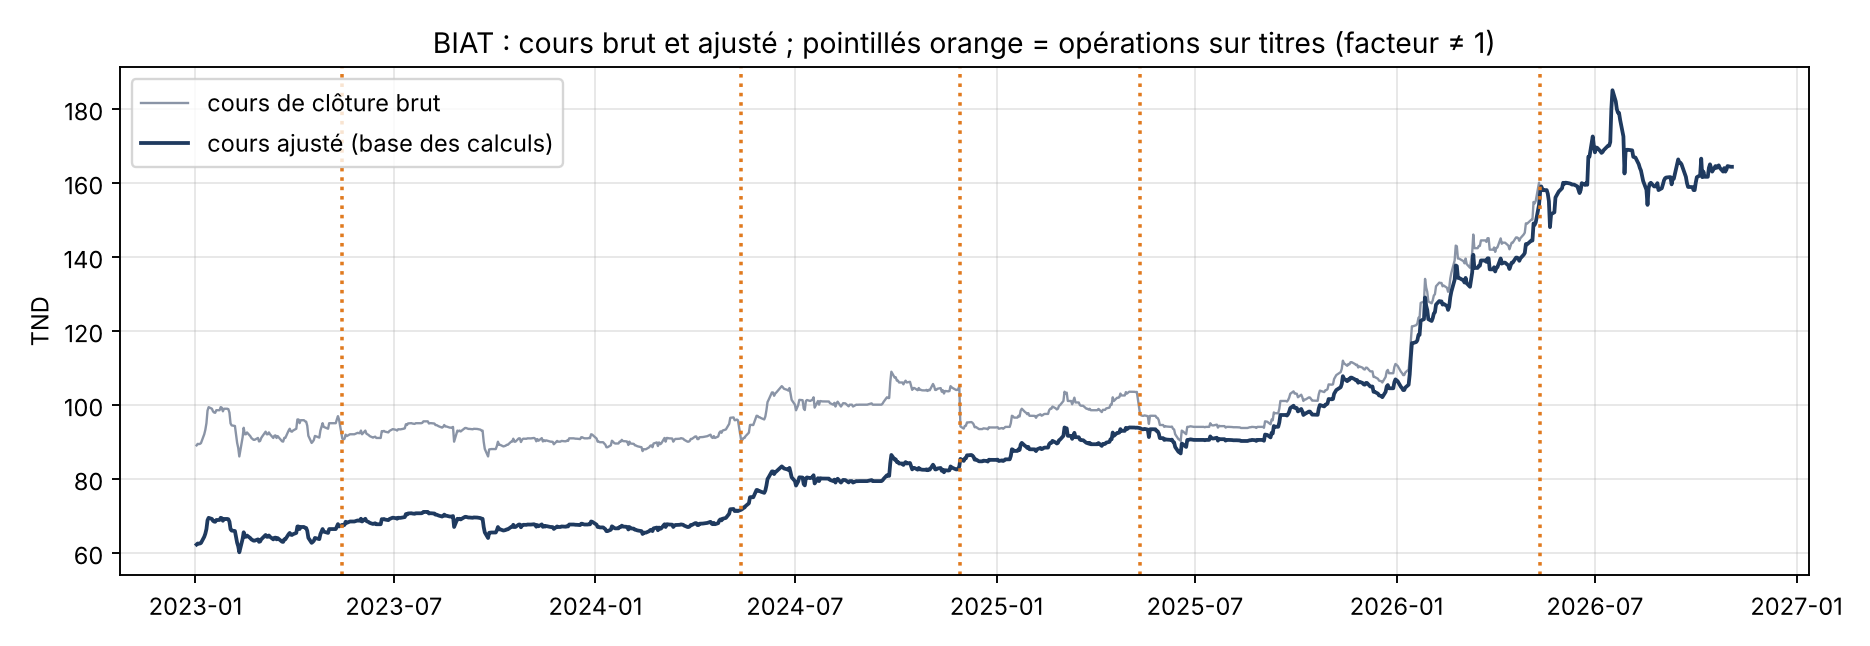
\includegraphics[width=\linewidth]{biat_brut_ajuste.png}
\caption{Cours brut et ajusté de BIAT. L'attribution gratuite de novembre 2024 faisait apparaître une fausse baisse d'environ 10\pc{} ; corrigée, la séance donne une hausse de 2,4\pc{}.}\label{fig:biat}
\end{figure}

\subsection{Qualité des données et limites connues}
\begin{itemize}
  \item les volumes de 2026 ne sont pas publiés dans les bulletins quotidiens ;
  \item une séance fictive (17/12/2025, jour férié) présente dans une source a été retirée ;
  \item \textbf{biais du survivant} : les dix sociétés radiées depuis 2023 sont hors univers ;
  \item certaines opérations sont classées « probables » quand leur nature exacte ne peut pas être confirmée par la source.
\end{itemize}

\section{Ce que nous ne reprenons pas de l'article}\label{sec:non-repris}
\begin{table}[H]\centering\small
\caption{Éléments de l'article non repris, et pourquoi}\label{tab:non-repris}
\begin{tabular}{p{5.5cm}p{8.5cm}}\toprule
Dans l'article & Chez nous \\ \midrule
VWAP et modèles multifacteurs & Le cours de clôture et le cours de référence officiel suffisent \\
Deux périodes Covid & Une seule période récente, 2023-2026 \\
100\,000 portefeuilles aléatoires & Optimisation exacte ; tirages aléatoires seulement comme contrôle \\
Autres algorithmes, scraping de la presse & Hors du cœur du travail ; la nature des anomalies est jugée sur des critères mesurables \\
\bottomrule\end{tabular}
\end{table}
Nous reproduisons le cœur de l'article, pas ses à-côtés.

\section{Nos paramètres}\label{sec:features}
\subsection{Définitions}
Pour un titre, le rendement journalier logarithmique est calculé à partir du cours de référence :
\begin{equation}
r_t = \ln\!\left(\frac{\text{clôture}_t}{\text{référence}_t}\right).
\end{equation}
Sur les $T = 959$ rendements, avec $\bar r$ la moyenne et $s$ l'écart-type :
\begin{align}
\text{Rendement} &= 252\,\bar r, & \text{Volatilité} &= \sqrt{252}\; s, \\
\text{Skewness} &= \frac{1}{T}\sum_t \left(\frac{r_t-\bar r}{s}\right)^{3}, & \text{Kurtosis} &= \frac{1}{T}\sum_t \left(\frac{r_t-\bar r}{s}\right)^{4} - 3,
\end{align}
\begin{equation}
\text{VaR}_{95} = q_{5\%}(r), \qquad \text{CVaR}_{95} = \mathbb{E}\left[\,r \mid r \leq \text{VaR}_{95}\right], \qquad
\beta = \frac{\operatorname{Cov}(r, r_M)}{\operatorname{Var}(r_M)},
\end{equation}
où $r_M$ est le rendement du Tunindex. VaR et CVaR sont historiques et journalières. On obtient \textbf{une valeur par titre sur toute la période}, soit un tableau de 75 titres $\times$ 7 features (annexe~\ref{ann:features}).

\subsection{Description}
\begin{table}[H]\centering\small
\caption{Statistiques des 7 features sur les 75 titres}\label{tab:desc-features}
\begin{tabular}{lrrrrrrr}\toprule
 & Rendement & Volatilité & Skewness & Kurtosis & VaR & CVaR & Bêta \\ \midrule
Moyenne & 15,3\pc{} & 26,0\pc{} & 0,47 & 6,04 & $-2{,}6$\pc{} & $-3{,}5$\pc{} & 0,43 \\
Médiane & 17,2\pc{} & 24,3\pc{} & 0,26 & 2,83 & $-2{,}4$\pc{} & $-3{,}8$\pc{} & 0,40 \\
Minimum & $-39{,}1$\pc{} & 4,8\pc{} & $-0{,}78$ & $-0{,}95$ & $-4{,}5$\pc{} & $-5{,}1$\pc{} & $-0{,}19$ \\
Maximum & 59,4\pc{} & 41,2\pc{} & 11,73 & 164,31 & 0,0\pc{} & 0,0\pc{} & 1,56 \\
\bottomrule\end{tabular}
\end{table}
Exemple : la SFBT a un rendement annualisé de 8,8\pc{}, une volatilité de 16,8\pc{} et un bêta de 0,82. Le Tunindex, lui, a un rendement de 22,0\pc{} par an pour une volatilité de 7,6\pc{}. Les valeurs extrêmes viennent des titres peu liquides : PLTU a un kurtosis de 164 et une VaR nulle, car 98\pc{} de ses rendements sont nuls.

\subsection{Corrélations entre features}
\begin{figure}[H]\centering
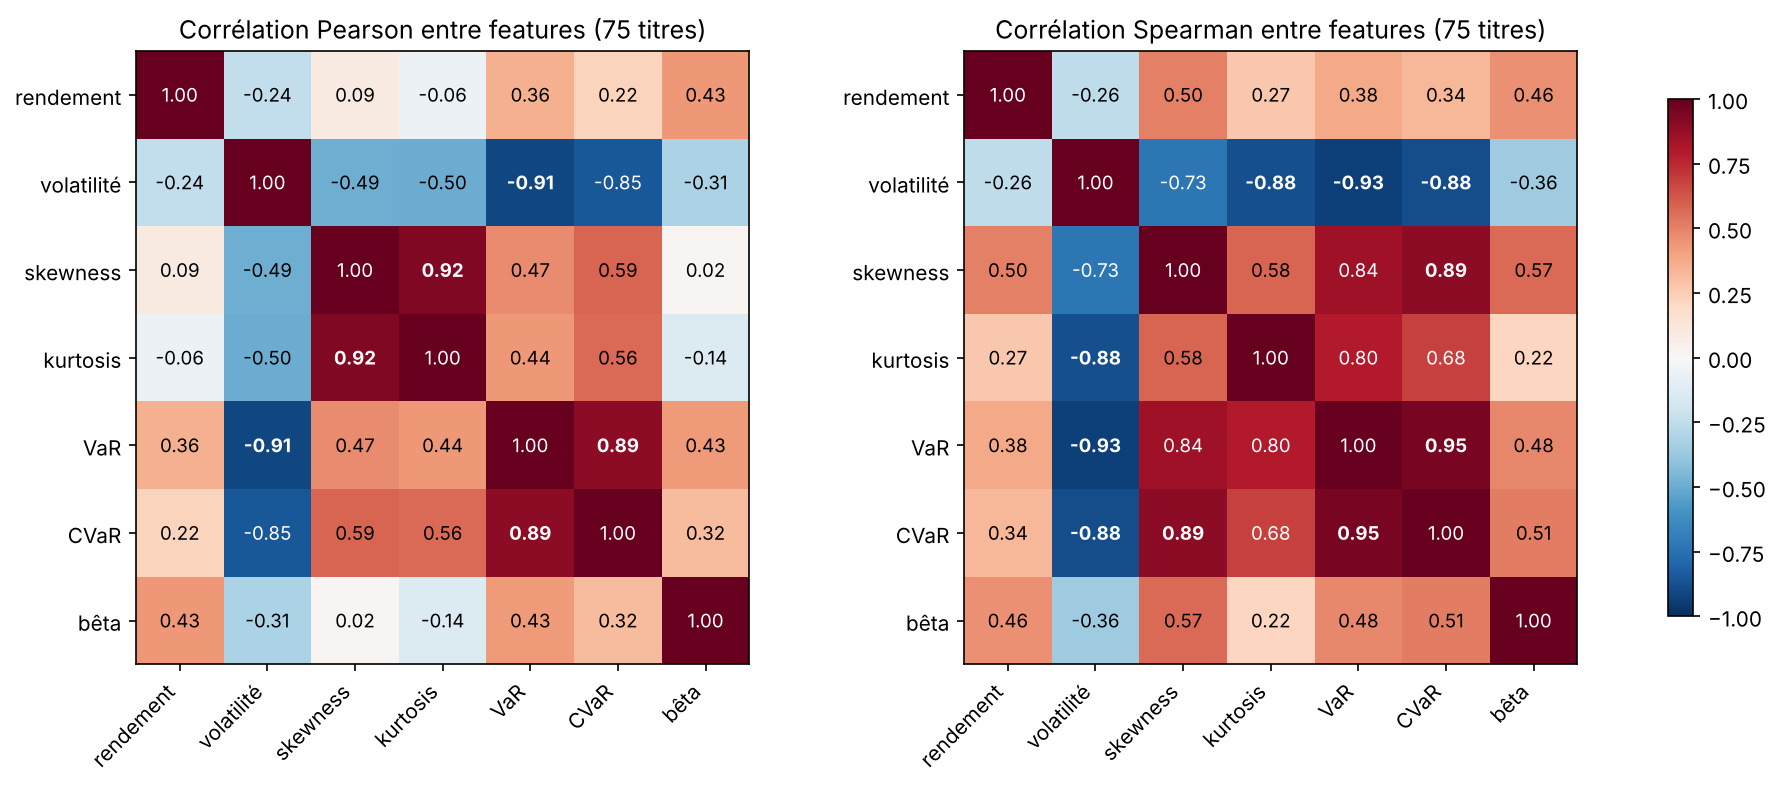
\includegraphics[width=\linewidth]{s4b_correlations_features.png}
\caption{Corrélations de Pearson et de Spearman entre les 7 features, calculées sur les 75 titres.}\label{fig:correlations}
\end{figure}
Deux paires sont presque des doublons : skewness et kurtosis (0,92 en Pearson), VaR et CVaR (0,89 en Pearson, 0,95 en Spearman). La volatilité est aussi fortement liée à la VaR ($-0{,}91$) et à la CVaR ($-0{,}85$). La section~\ref{sec:5f} examine l'effet de cette redondance sur les résultats.

\section{Markowitz sur nos données}\label{sec:markowitz}
\subsection{Taux sans risque}
Nous prenons le taux du marché monétaire (TMM) d'octobre 2026, égal au taux directeur de la Banque centrale de Tunisie : 7\pc{}. Comme nos rendements sont logarithmiques, nous le convertissons en taux continu : $r_f = \ln(1{,}07) = 6{,}77\pc{}$. Sur les 75 titres, 51 ont un rendement annualisé supérieur à $r_f$.

\subsection{Méthode exacte}
Avec $\mu$ le vecteur des rendements annualisés et $\Sigma$ la covariance annualisée (rendements journaliers, $\times 252$), un portefeuille de poids $w$ a pour rendement $\mu^\top w$, pour volatilité $\sqrt{w^\top \Sigma w}$ et pour ratio de Sharpe $(\mu^\top w - r_f)/\sqrt{w^\top\Sigma w}$. La matrice $\Sigma$ est symétrique et définie positive (conditionnement 98).

\paragraph{Variance minimale.} La forme fermée, qui autorise la vente à découvert, est
\begin{equation}
w_{\text{GMV}} = \frac{\Sigma^{-1}\mathbf{1}}{\mathbf{1}^\top \Sigma^{-1}\mathbf{1}}.
\end{equation}
Nous calculons aussi la version sans vente à découvert, plus réaliste à la BVMT : $\min_w w^\top\Sigma w$ sous $\mathbf{1}^\top w = 1$, $w \geq 0$.

\paragraph{Sharpe maximal.} Sans vente à découvert, nous utilisons le changement de variable de Cornuéjols et Tütüncü (2007) :
\begin{equation}
\min_{y \geq 0}\; y^\top \Sigma y \quad \text{sous} \quad (\mu - r_f\mathbf{1})^\top y = 1, \qquad\text{puis}\qquad w = \frac{y}{\mathbf{1}^\top y}.
\end{equation}
Le problème est convexe : la solution trouvée est l'optimum global.

\paragraph{Frontière efficiente.} Elle part du portefeuille de variance minimale (rendement 9,0\pc{}) et va jusqu'au titre de plus haut rendement (SOTET, 59,4\pc{}). Pour 40 rendements cibles $m$ régulièrement espacés, on résout $\min_w w^\top\Sigma w$ sous $\mathbf{1}^\top w = 1$, $\mu^\top w = m$, $w \geq 0$ (SLSQP). Avec le portefeuille de Sharpe maximal, cela donne 41 portefeuilles.

\subsection{Résultats}
\begin{figure}[H]\centering
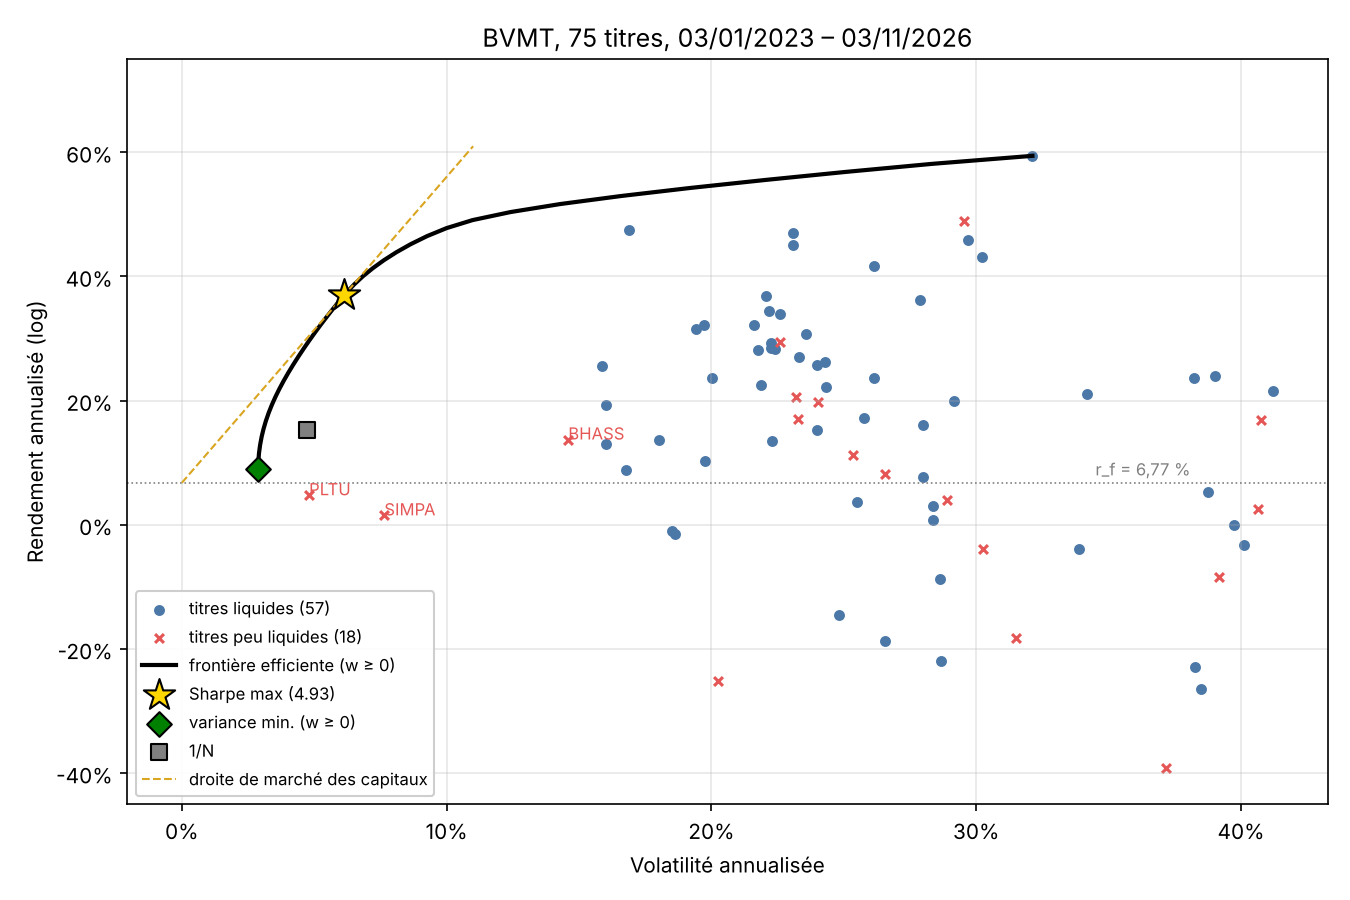
\includegraphics[width=0.82\linewidth]{frontiere_efficiente.png}
\caption{Frontière efficiente sans vente à découvert, 75 titres. Étoile : Sharpe maximal ; losange : variance minimale ; carré : 1/N ; pointillés : droite de marché des capitaux.}\label{fig:frontiere}
\end{figure}

\begin{table}[H]\centering\small
\caption{Portefeuilles de Markowitz : 75 titres et 57 titres liquides}\label{tab:markowitz}
\begin{tabular}{llrrrl}\toprule
Univers & Portefeuille & Rendement & Volatilité & Sharpe & Premier poids \\ \midrule
75 titres & Variance min.\ (forme fermée) & 8,9\pc{} & 2,9\pc{} & 0,74 & PLTU (37\pc{}) \\
 & Variance min.\ ($w \geq 0$) & 9,0\pc{} & 2,9\pc{} & 0,77 & PLTU (37\pc{}) \\
 & Sharpe max.\ ($w \geq 0$) & \textbf{36,9\pc{}} & \textbf{6,1\pc{}} & \textbf{4,93} & AB (10\pc{}) \\
 & 1/N & 15,3\pc{} & 4,7\pc{} & 1,80 & — \\ \midrule
57 liquides & Variance min.\ (forme fermée) & 15,7\pc{} & 4,8\pc{} & 1,88 & WIFAK (7\pc{}) \\
 & Variance min.\ ($w \geq 0$) & 16,2\pc{} & 4,8\pc{} & 1,96 & WIFAK (7\pc{}) \\
 & Sharpe max.\ ($w \geq 0$) & 38,3\pc{} & 7,0\pc{} & 4,52 & AB (13\pc{}) \\
 & 1/N & 18,3\pc{} & 5,6\pc{} & 2,08 & — \\
\bottomrule\end{tabular}
\end{table}

Le portefeuille de Sharpe maximal donne 4,93. Le meilleur de 20\,000 portefeuilles tirés au hasard n'atteint que 3,22 : l'optimisation exacte fait mieux que la simulation de l'article. Les poids détaillés sont en annexe~\ref{ann:poids}.

\subsection{Deux résultats à ne pas prendre au pied de la lettre}
\paragraph{Le piège de la variance minimale.} Le portefeuille de variance minimale met 37\pc{} sur PLTU et 14\pc{} sur SIMPA, deux titres échangés 4\pc{} et 12\pc{} des séances. Leur volatilité est faible parce que leur prix ne bouge presque jamais, pas parce qu'ils sont peu risqués. Ce portefeuille ne pourrait pas être acheté en pratique. Sur les 57 titres liquides, sa volatilité passe de 2,9\pc{} à 4,8\pc{}.

\paragraph{Un Sharpe de 4,93 n'est pas une performance réalisable.} Nous retrouvons un Sharpe du même ordre que celui de l'article, que nous avons critiqué. Trois effets le gonflent :
\begin{enumerate}
  \item \textbf{un marché très haussier} : le Tunindex a gagné 7,8\pc{}, 12,9\pc{}, 30,1\pc{} et 32,8\pc{} (en log) en 2023, 2024, 2025 et 2026 ;
  \item \textbf{une optimisation dans l'échantillon} : les poids sont choisis sur les mêmes données que celles qui servent à les évaluer ;
  \item \textbf{une volatilité sous-estimée} : les rendements journaliers sont autocorrélés (0,29 pour le Tunindex), car les prix s'ajustent avec retard. Avec une covariance hebdomadaire, la volatilité du Tunindex passe de 7,6\pc{} à 9,9\pc{} et le Sharpe du portefeuille optimal tombe de 4,93 à 3,70.
\end{enumerate}

\begin{retenir}
Markowitz exact donne les mêmes excès que l'article : des Sharpe irréalistes et un portefeuille de variance minimale piégé par l'illiquidité. Seul un test hors échantillon peut dire si une méthode diversifie vraiment.
\end{retenir}

\section{Segmentation et anomalies : notre méthode}\label{sec:methode}
\subsection{Préparation : standardisation et trois espaces}
Les features sont standardisées sur les 75 titres : $z = (x - \text{moyenne})/\text{écart-type}$. Sans cela, le kurtosis (jusqu'à 164) écraserait la VaR et la CVaR (quelques centièmes) dans les distances. Nous travaillons dans trois espaces :
\begin{itemize}
  \item \textbf{RV} : rendement et volatilité, le plan de l'article ;
  \item \textbf{7F} : les sept features ;
  \item \textbf{ACP} : les composantes principales qui expliquent au moins 80\pc{} de la variance.
\end{itemize}

\subsection{Analyse en composantes principales}
Trois composantes expliquent \textbf{89\pc{}} de la variance (54,5\pc{}, 23,9\pc{} et 10,5\pc{}). PC1 est un axe « risque » : VaR et CVaR d'un côté, volatilité de l'autre. PC2 oppose le bêta et le rendement au kurtosis et au skewness. PC3 est surtout porté par le rendement.

\begin{figure}[H]\centering
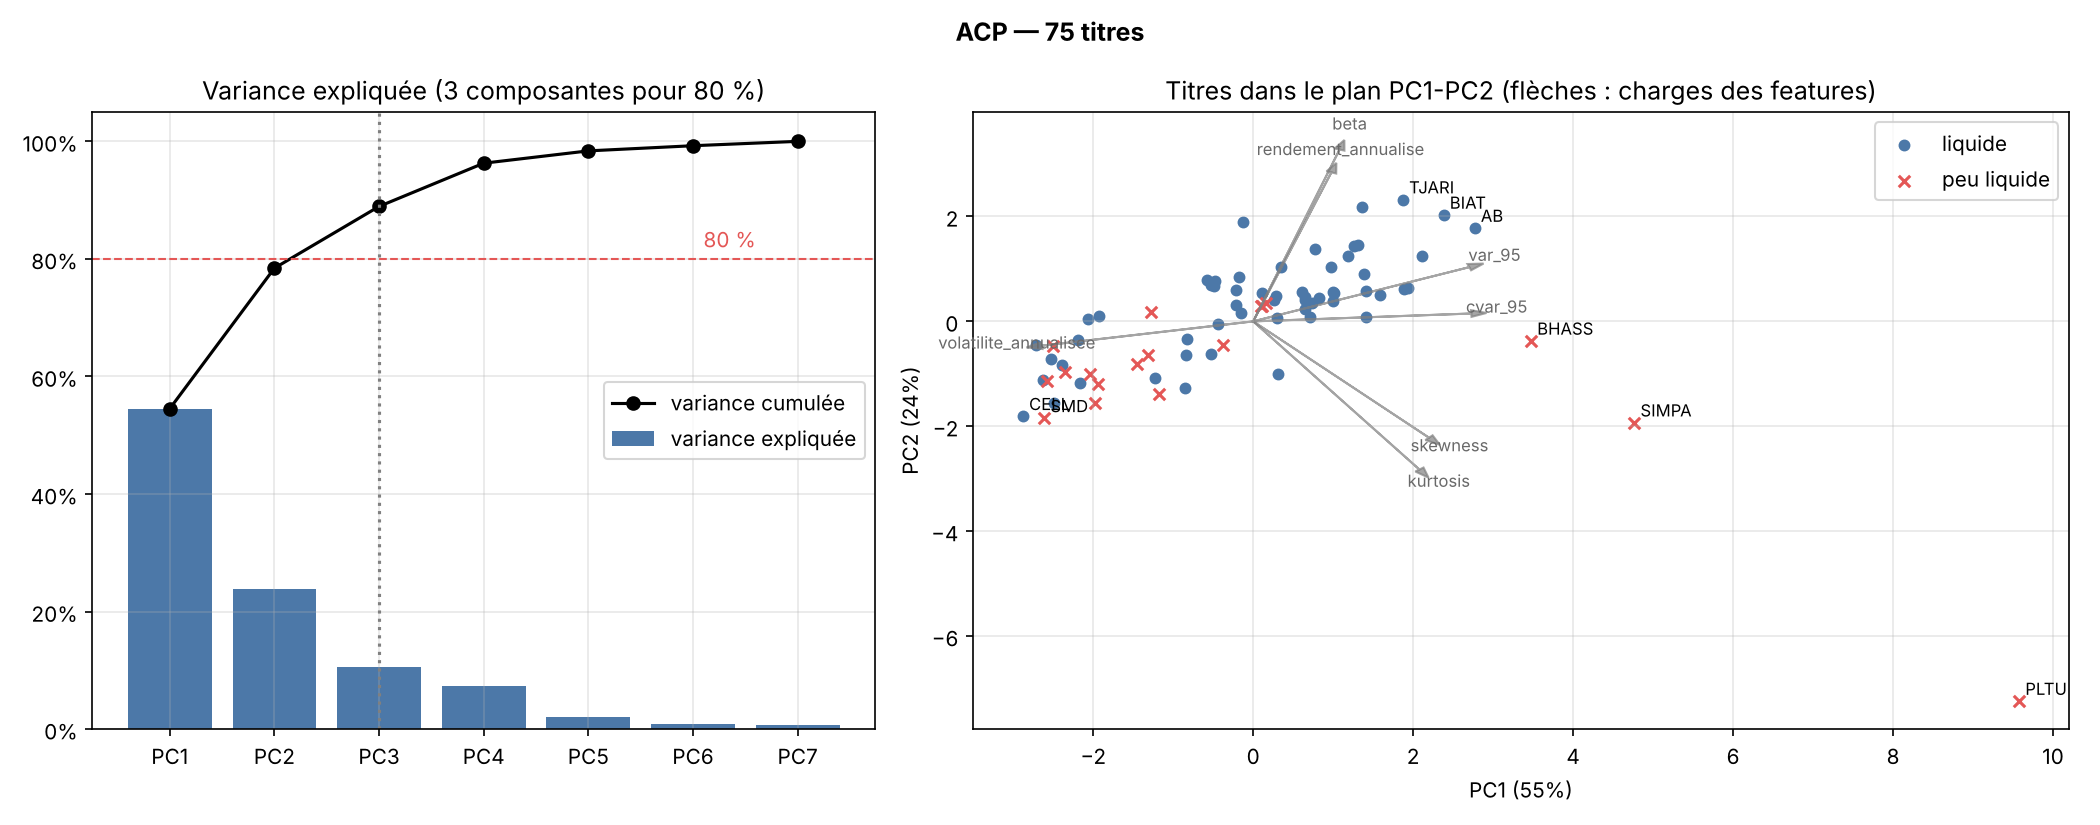
\includegraphics[width=\linewidth]{s4_acp.png}
\caption{ACP sur les 75 titres : variance expliquée et projection sur PC1-PC2.}\label{fig:acp}
\end{figure}

\subsection{K-means et choix de \texorpdfstring{$k$}{k}}
K-means cherche $k$ groupes qui minimisent l'inertie intra-groupe $\sum_{j=1}^{k}\sum_{x \in C_j}\lVert x - \mu_j\rVert^2$. Nous utilisons l'initialisation k-means++ (Arthur et Vassilvitskii, 2007), 50 initialisations et la graine 42. Pour $k$ de 3 à 8, quatre critères votent :

\begin{table}[H]\centering\small
\caption{Les quatre critères de choix de $k$}\label{tab:criteres}
\begin{tabular}{lp{7.6cm}l}\toprule
Critère & Ce qu'il mesure & Meilleur $k$ \\ \midrule
Coude & Point où ajouter un groupe ne fait plus beaucoup baisser l'inertie & courbure maximale \\
Silhouette & $s(i) = \dfrac{b(i)-a(i)}{\max(a(i),b(i))}$ : ressemblance d'un titre à son groupe ($a$) comparée au groupe voisin ($b$), entre $-1$ et 1 & la plus haute \\
Calinski-Harabasz & Dispersion entre les groupes rapportée à la dispersion dans les groupes & le plus haut \\
Davies-Bouldin & Ressemblance moyenne de chaque groupe à son plus proche voisin & le plus bas \\
\bottomrule\end{tabular}
\end{table}

On retient le $k$ qui a le plus de votes ; en cas d'égalité, la silhouette tranche. On signale tout $k$ au bord de la plage, tout groupe d'un seul titre et toute silhouette inférieure à 0,5.

\subsection{Isolation Forest}
Isolation Forest (Liu, Ting et Zhou, 2008) construit des arbres de découpes aléatoires : un point anormal s'isole en peu de découpes. Son score est
\begin{equation}
s(x) = 2^{-\mathbb{E}[h(x)]/c(n)}, \qquad c(n) = 2H(n-1) - \frac{2(n-1)}{n},
\end{equation}
où $h(x)$ est la profondeur à laquelle $x$ est isolé et $H$ le nombre harmonique. Nous utilisons 500 arbres et la graine 42. Le taux de contamination ne change pas les scores, seulement le seuil : nous le testons à 3, 5, 8 et 10\pc{} et retenons 5\pc{}, comme l'article. Avec trois espaces et quatre taux, chaque titre passe \textbf{12 tests} ; une \textbf{anomalie stable} est un titre signalé au moins 8 fois sur 12.

\subsection{Nature de chaque anomalie}
Une même règle est appliquée à chaque titre signalé :
\begin{itemize}
  \item \textbf{artefact d'illiquidité} s'il est échangé moins de 60\pc{} des séances ou a plus de 50\pc{} de rendements nuls ;
  \item sinon, \textbf{performance extrême} si au moins une feature est à plus de 2 écarts-types de la moyenne ;
  \item sinon, \textbf{atypique modéré} : le titre est isolé par une combinaison de features.
\end{itemize}
Aucune anomalie n'est présentée comme une société en difficulté : ce jugement demanderait une preuve externe (états financiers, communiqués du CMF ou de la BVMT). Enfin, \textbf{tout est refait sur les 57 titres liquides}, standardisation et ACP comprises.

\section{Nos résultats : les clusters}\label{sec:clusters}
\subsection{Choix de \texorpdfstring{$k$}{k}}
\begin{table}[H]\centering\small
\caption{Votes des quatre critères et $k$ retenu, 75 titres}\label{tab:votes}
\begin{tabular}{lccccccl}\toprule
Espace & Coude & Silhouette & CH & DB & $k$ retenu & Silhouette & Tailles \\ \midrule
RV & 5 & 8 & 8 & 8 & \textbf{8} & 0,441 & 22 / 13 / 11 / 9 / 8 / 7 / 3 / 2 \\
7F & 5 & 3 & 3 & 3 & \textbf{3} & 0,406 & 48 / 26 / 1 \\
ACP & 5 & 3 & 8 & 3 & \textbf{3} & 0,469 & 47 / 27 / 1 \\
\bottomrule\end{tabular}
\end{table}

\begin{figure}[H]\centering
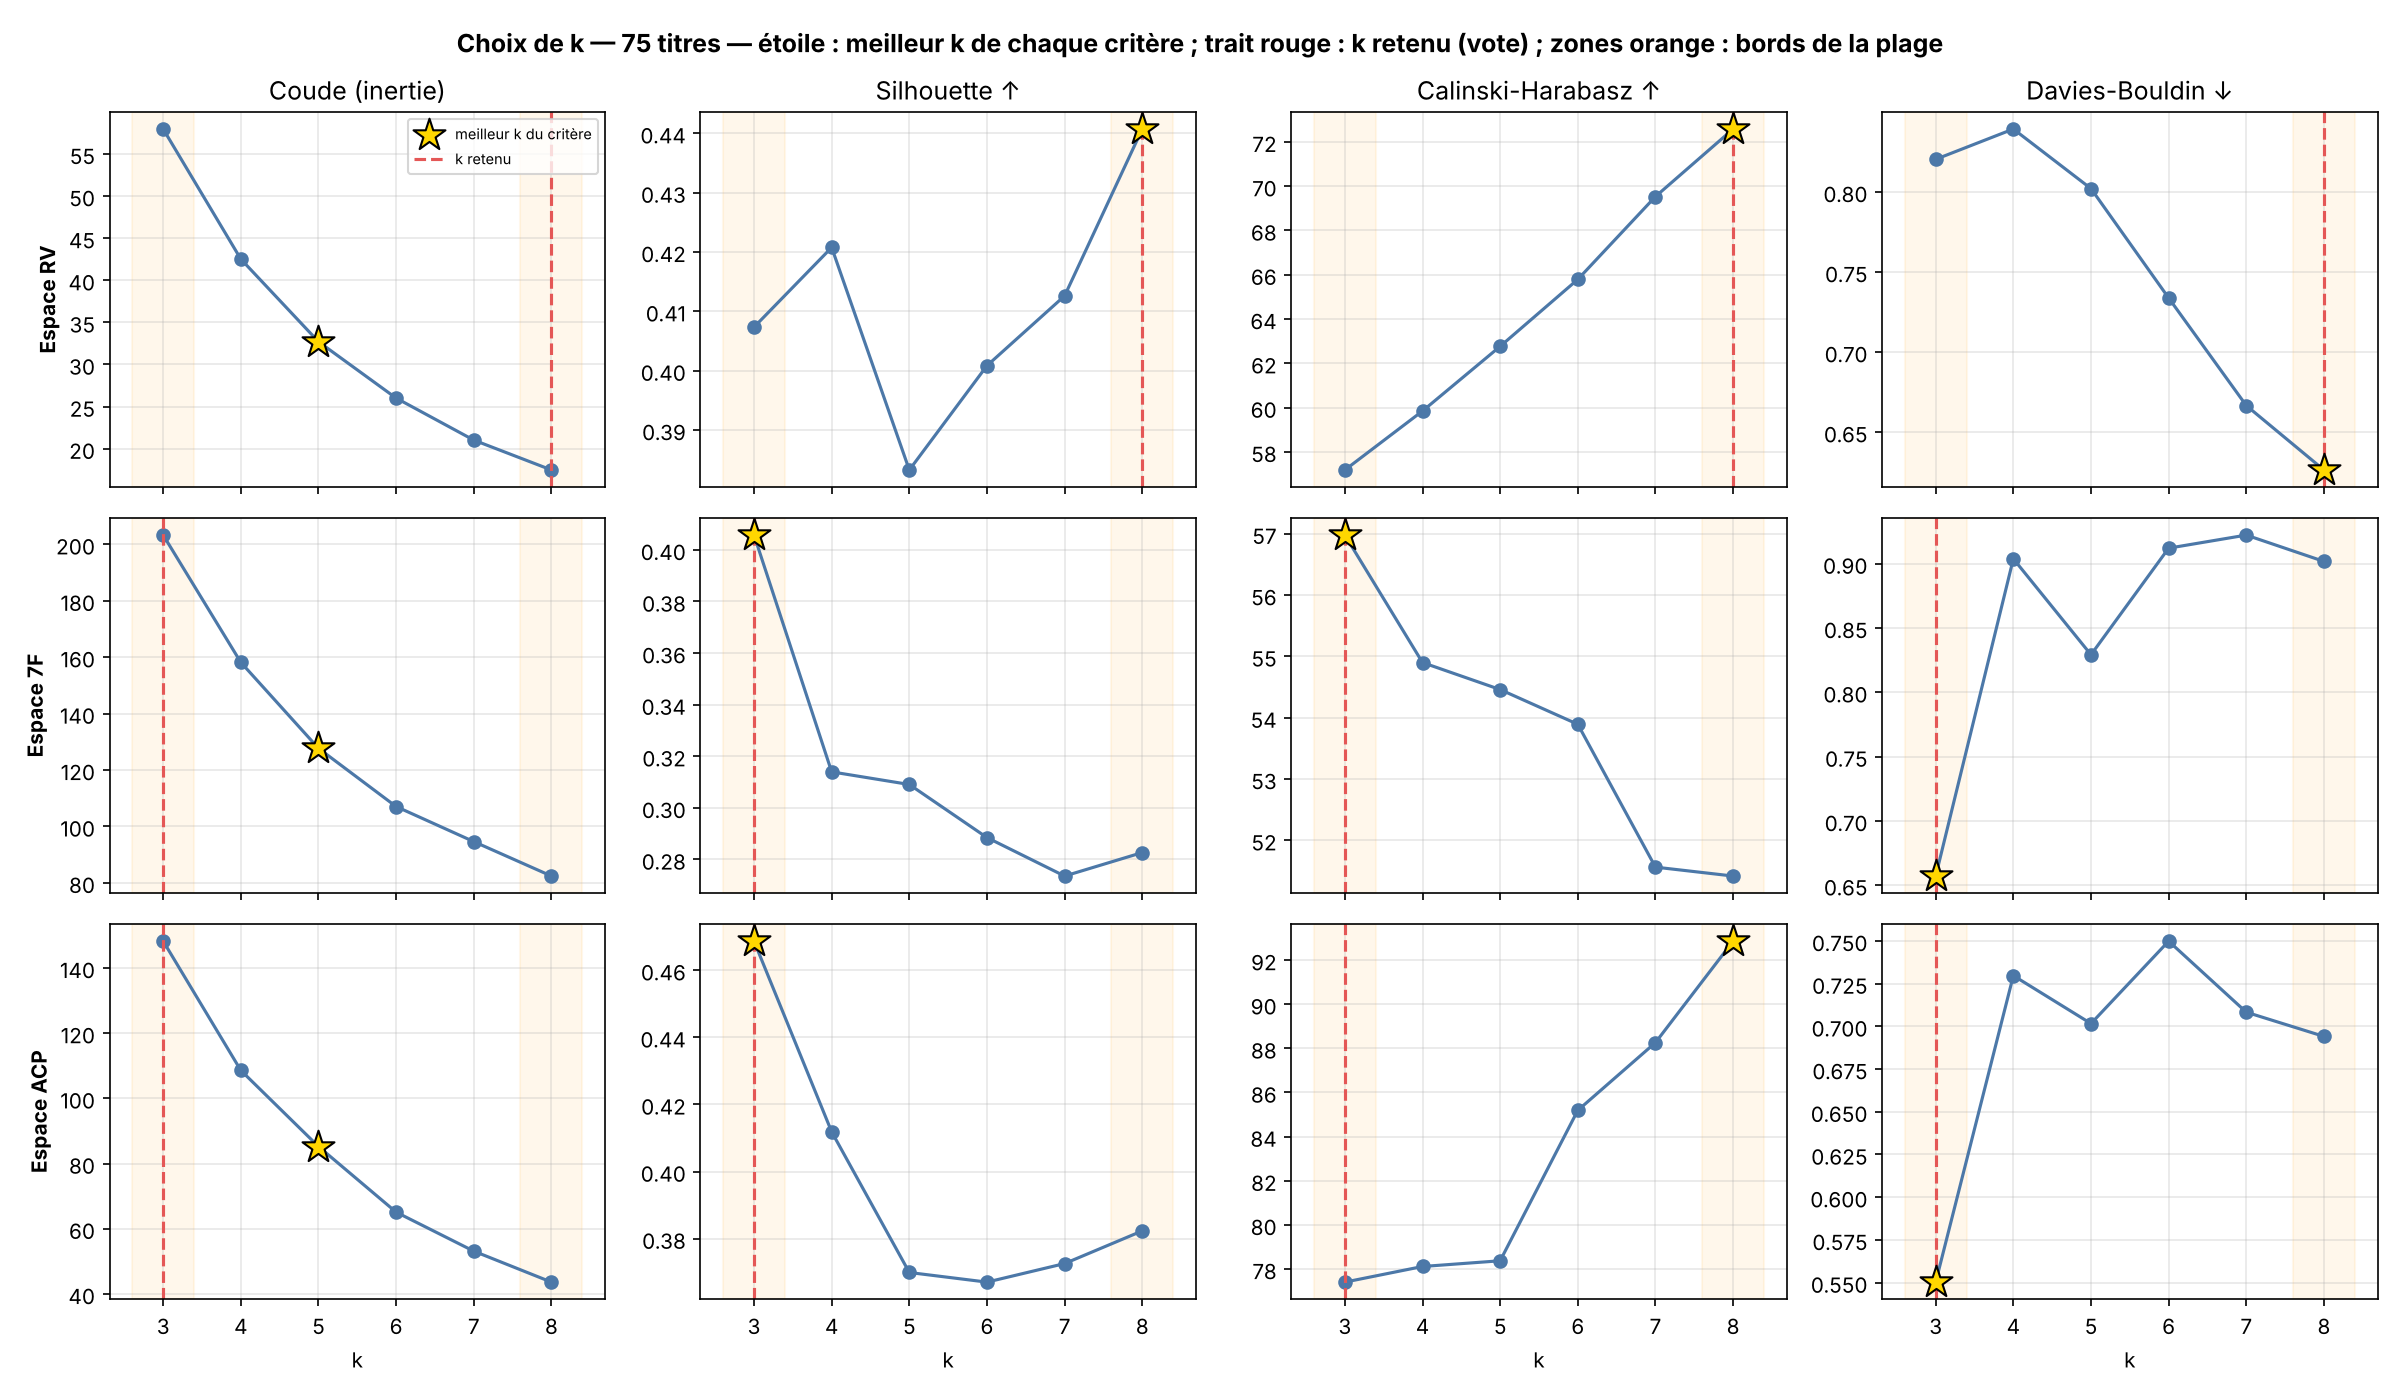
\includegraphics[width=\linewidth]{s4_choix_k.png}
\caption{Les quatre critères pour $k$ de 3 à 8 dans les trois espaces. Étoile : meilleur $k$ de chaque critère ; trait rouge : $k$ retenu.}\label{fig:choix-k}
\end{figure}

\paragraph{Plan rendement-volatilité : $k = 8$.} Trois critères sur quatre votent pour 8, la limite haute de la plage. Ces critères s'améliorent presque à chaque groupe ajouté, car le plan forme un nuage continu, sans groupes naturels : plus on le découpe, plus les morceaux sont compacts. Hors de la plage, la silhouette vaut d'ailleurs 0,46 à $k = 9$ et à $k = 12$. \textbf{$k = 8$ n'est donc pas un vrai optimum} : le plan de l'article ne contient pas de structure claire (silhouette de 0,38 à 0,44 pour $k$ de 3 à 8).

\paragraph{Sept features : $k = 3$.} Trois critères sur quatre votent pour 3, et c'est un vrai optimum : $k = 2$ donne une silhouette plus basse (0,38), de même que $k = 9$ à 12 (0,26 à 0,29). L'espace ACP donne le même résultat ($k = 3$, silhouette 0,47 contre 0,44 à $k = 2$).

\paragraph{Pourquoi la plage 3 à 8.} $k = 2$ ne permettrait pas de diversifier entre groupes (un portefeuille « un titre par groupe » n'aurait que deux titres), et au-delà de 8 groupes, avec 75 titres, les groupes deviennent minuscules et instables. La plage encadre le $k = 7$ de l'article.

\subsection{Les groupes}
\begin{figure}[H]\centering
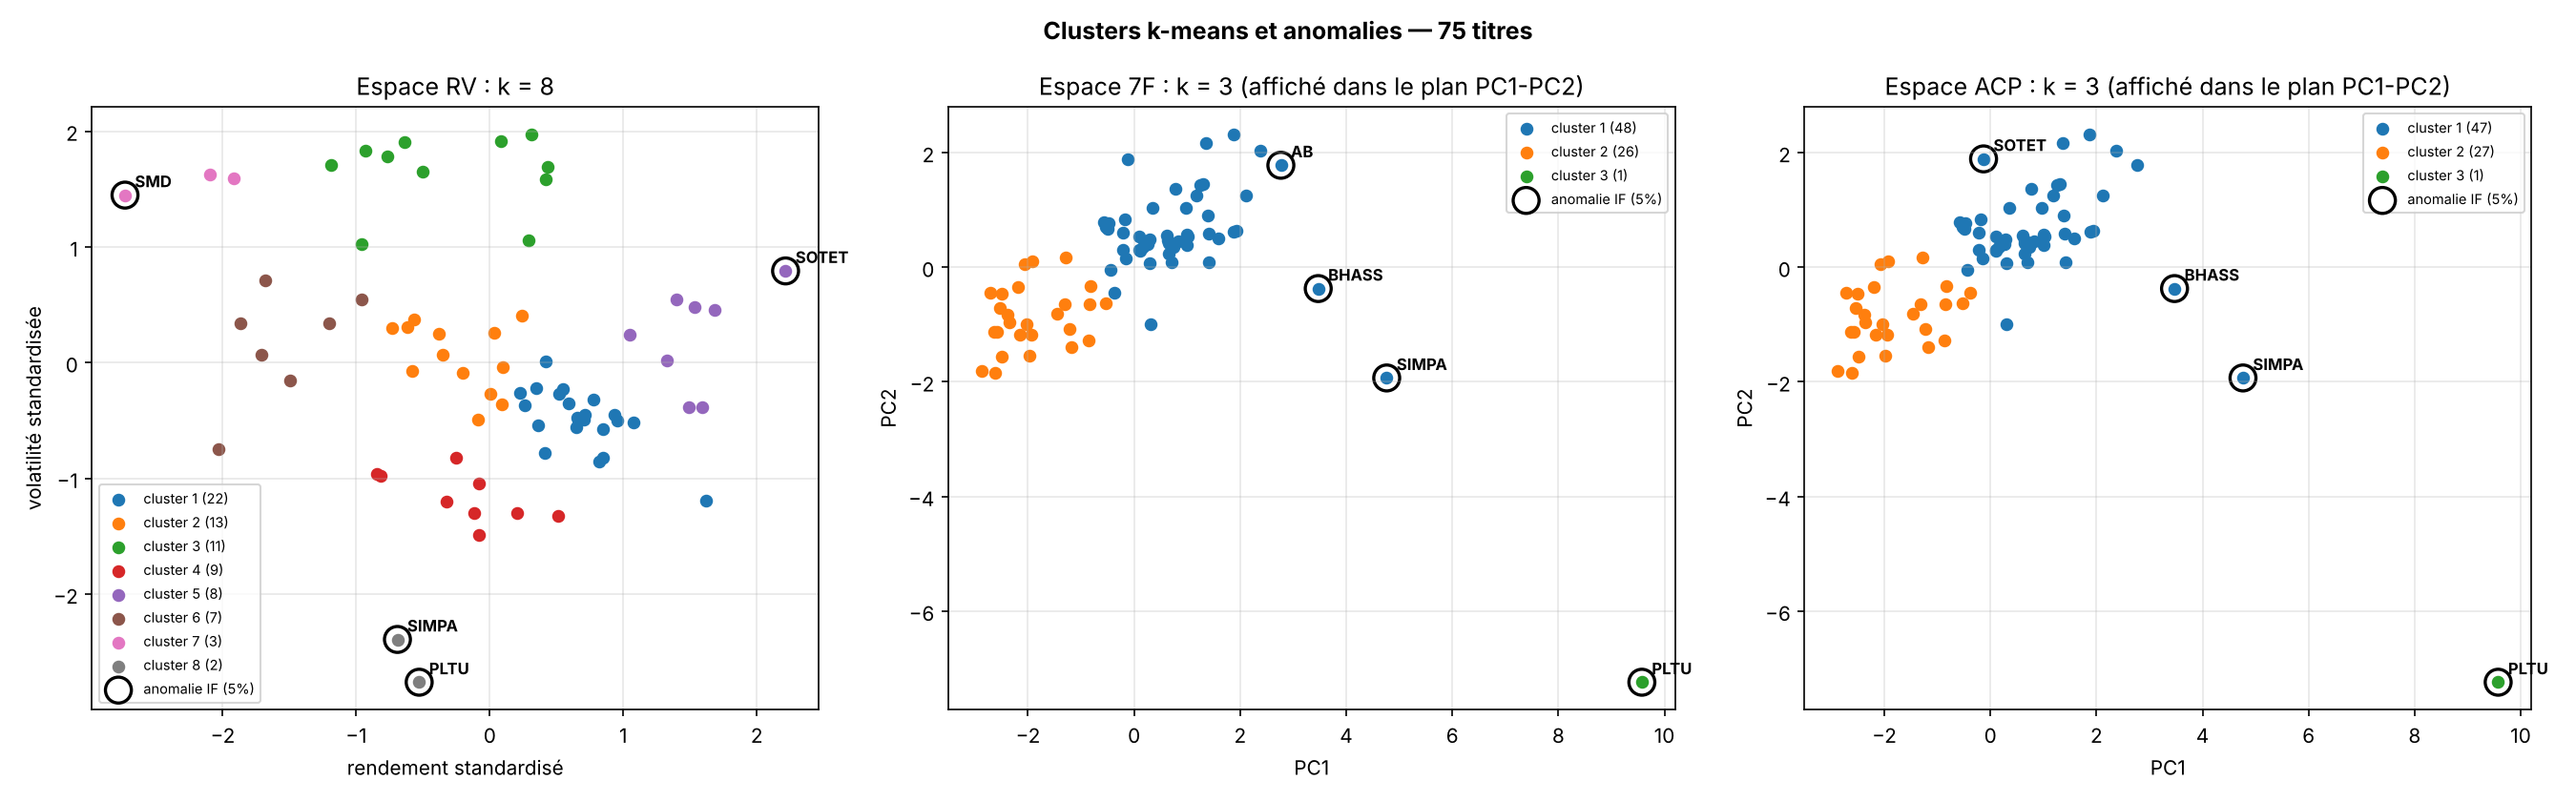
\includegraphics[width=\linewidth]{s4_clusters.png}
\caption{Groupes k-means dans les trois espaces (7F et ACP affichés dans le plan PC1-PC2) ; cercles : anomalies Isolation Forest à 5\pc{}.}\label{fig:clusters}
\end{figure}

\begin{table}[H]\centering\small
\caption{Profil des groupes, espace 7F (médianes)}\label{tab:profil-7f}
\begin{tabular}{lrrrrrrr}\toprule
Groupe & Taille & Rendement & Volatilité & Bêta & Séances échangées & Capitaux médians (TND) & Peu liquides \\ \midrule
1 & 48 & 24,6\pc{} & 22,6\pc{} & 0,58 & 95\pc{} & 13\,956 & 6 \\
2 & 26 & $-1{,}6$\pc{} & 34,0\pc{} & 0,13 & 69\pc{} & 115 & 11 \\
3 (PLTU) & 1 & 4,8\pc{} & 4,8\pc{} & 0,00 & 4\pc{} & 0 & 1 \\
\bottomrule\end{tabular}
\end{table}

\begin{itemize}
  \item \textbf{Groupe 1 (48 titres)} : titres liquides et liés au marché, avec toutes les banques sauf BTE (AB, ATB, BH, BIAT, BNA, BT, STB, UBCI, UIB, Attijari, Wifack).
  \item \textbf{Groupe 2 (26 titres)} : titres volatils, à rendement proche de zéro et peu liés au marché, dont les capitaux échangés sont environ \textbf{120 fois plus petits}.
  \item \textbf{Groupe 3 : PLTU seule}, isolée quel que soit $k$ par son skewness extrême et ses prix figés.
\end{itemize}

\begin{retenir}
Les groupes ne sont pas des secteurs : ils séparent un monde liquide et lié au marché d'un monde volatil, peu échangé et peu lié au marché. La structure est faible partout (silhouette inférieure à 0,5).
\end{retenir}

\subsection{Sur les 57 titres liquides}
Sans les titres peu liquides, le vote retient $k = 8$ (RV), $k = 3$ (7F, groupes de 23 / 23 / 11) et $k = 5$ (ACP), avec des silhouettes de 0,47, 0,31 et 0,39. L'accord avec la partition des 75 titres, mesuré par l'indice de Rand ajusté (ARI) sur les 57 titres communs, est élevé dans le plan RV (0,93) mais faible avec 7 features (0,34) et après ACP (0,26) : une fois les titres illiquides retirés, la partition change beaucoup, ce qui confirme que la liquidité structurait les groupes.

\section{Nos résultats : les anomalies}\label{sec:anomalies}
\begin{figure}[H]\centering
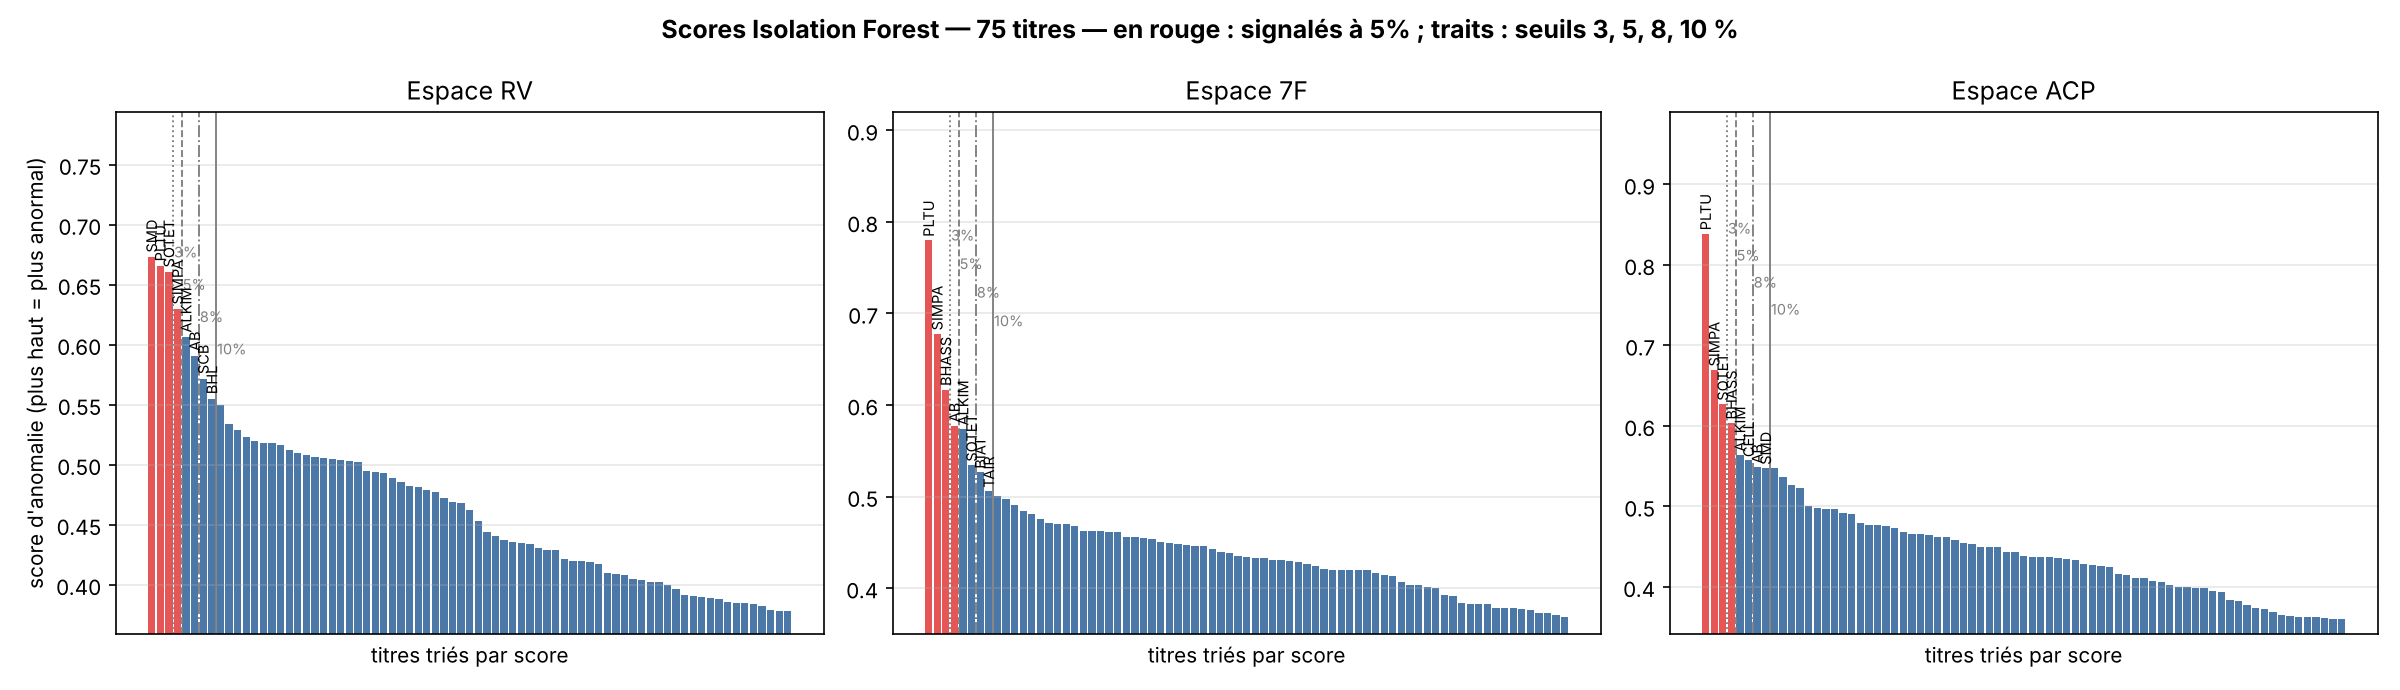
\includegraphics[width=\linewidth]{s4_scores_isolation_forest.png}
\caption{Scores Isolation Forest triés dans les trois espaces ; en rouge, les titres signalés à 5\pc{}.}\label{fig:scores-if}
\end{figure}

\begin{table}[H]\centering\small
\caption{Titres signalés au moins cinq fois sur 12 tests, 75 titres}\label{tab:anomalies}
\begin{tabular}{llrrrl}\toprule
Titre & Nom & Signalements & Séances échangées & Rendement & Nature \\ \midrule
PLTU & Placements de Tunisie SICAF & \textbf{12} & 4\pc{} & 4,8\pc{} & artefact d'illiquidité \\
SIMPA & SIMPAR & \textbf{11} & 12\pc{} & 1,5\pc{} & artefact d'illiquidité \\
SOTET & SOTETEL & \textbf{10} & 99\pc{} & 59,4\pc{} & performance extrême (hausse) \\
BHASS & BH Assurance & 7 & 10\pc{} & 13,7\pc{} & artefact d'illiquidité \\
AB & Amen Bank & 6 & 99\pc{} & 47,5\pc{} & atypique modéré \\
ALKIM & Alkimia & 6 & 18\pc{} & $-25{,}2$\pc{} & artefact d'illiquidité \\
SMD & Sanimed & 5 & 27\pc{} & $-39{,}1$\pc{} & artefact d'illiquidité \\
\bottomrule\end{tabular}
\end{table}

\begin{itemize}
  \item \textbf{Trois anomalies stables} : PLTU (12 sur 12), SIMPA (11) et SOTET (10).
  \item \textbf{PLTU, SIMPA et BHASS sont des artefacts d'illiquidité} : échangés 4 à 12\pc{} des séances, avec plus de 90\pc{} de rendements nuls. L'algorithme ne trouve pas des sociétés en difficulté, il trouve des prix qui ne bougent pas.
  \item \textbf{SOTET et AB sont de vrais extrêmes de performance}, avec 59\pc{} et 47\pc{} de rendement annualisé, à confirmer avec des sources externes.
  \item \textbf{Sur les 57 titres liquides}, les anomalies stables sont AB (9 sur 12), SOTET (8) et WIFAK (8). WIFAK, échangée 69\pc{} des séances, a 61\pc{} de rendements nuls : elle relève encore de l'illiquidité.
\end{itemize}
Le détail des titres signalés à chaque taux est en annexe~\ref{ann:stabilite}.

\begin{retenir}
La plupart des anomalies viennent de l'illiquidité. L'article validait ses anomalies par la presse sans contrôler la liquidité : une partie d'entre elles pourrait relever du même artefact.
\end{retenir}

\section{Contrôle de robustesse : cinq features sans redondance}\label{sec:5f}
\subsection{Pourquoi retirer deux features}
Garder deux features presque identiques revient à compter deux fois la même information dans les distances de k-means et d'Isolation Forest. Dans chaque paire redondante (skewness / kurtosis à 0,92 ; VaR / CVaR à 0,89), nous retirons la feature la plus corrélée, en moyenne, aux cinq autres :

\begin{table}[H]\centering\small
\caption{Choix de la feature retirée dans chaque paire redondante}\label{tab:choix-5f}
\begin{tabular}{lccccl}\toprule
Paire & Pearson & Spearman & Corr.\ moyenne aux autres & Retirée & Autre raison \\ \midrule
Skewness / kurtosis & 0,92 & 0,58 & 0,330 / 0,339 & kurtosis & dominé par PLTU (164) \\
VaR / CVaR & 0,89 & 0,95 & 0,521 / 0,508 & VaR & la CVaR est cohérente \\
\bottomrule\end{tabular}
\end{table}

Les écarts de corrélation moyenne sont faibles ; d'autres raisons vont dans le même sens. Le skewness garde le sens de l'asymétrie, que le kurtosis ne donne pas, et la CVaR est une mesure de risque \emph{cohérente} au sens d'Artzner et al.\ (1999), qui regarde toute la queue des pertes. Il reste \textbf{rendement, volatilité, skewness, CVaR et bêta}. La corrélation volatilité / CVaR ($-0{,}85$) est gardée volontairement : la première mesure les variations ordinaires, la seconde les pertes extrêmes.

\subsection{Résultats}
\begin{figure}[H]\centering
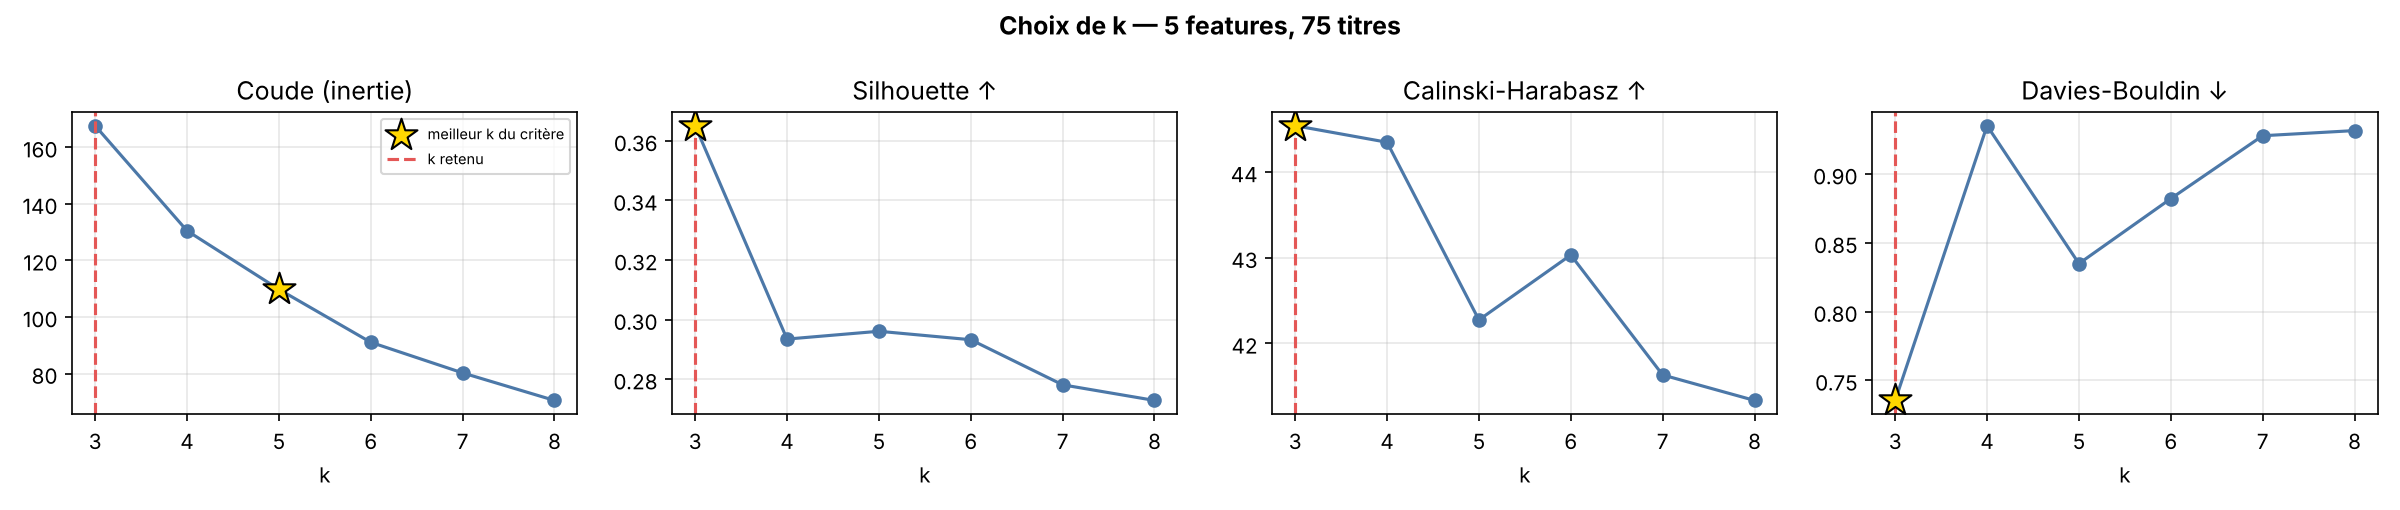
\includegraphics[width=\linewidth]{s4b_choix_k.png}
\caption{Choix de $k$ avec 5 features, 75 titres.}\label{fig:choix-k-5f}
\end{figure}

\begin{itemize}
  \item \textbf{$k = 3$ est confirmé} : silhouette, Calinski-Harabasz et Davies-Bouldin votent pour 3. C'est un vrai optimum ($k = 2$ : 0,343 ; $k = 9$ et 10 : 0,26 et 0,30). La silhouette, 0,365, est un peu plus basse qu'avec 7 features (0,406) : la redondance créait une partie de la séparation.
  \item \textbf{Les mêmes groupes} : 46 titres liquides et liés au marché (rendement médian 26\pc{}, volatilité 23\pc{}, bêta 0,59), 28 titres volatils et peu liés au marché (rendement $-0{,}7$\pc{}, volatilité 33\pc{}, bêta 0,13), et PLTU seule.
  \item \textbf{Les deux partitions sont très proches} : ARI de 0,80 avec la partition à 7 features ; seuls 4 titres sur 75 changent de groupe (AST, ICF et WIFAK passent au groupe 2, TINV au groupe 1).
  \item \textbf{Les mêmes anomalies} à 5\pc{} : AB, BHASS, PLTU et SIMPA, exactement celles de l'espace 7F.
\end{itemize}

\begin{figure}[H]\centering
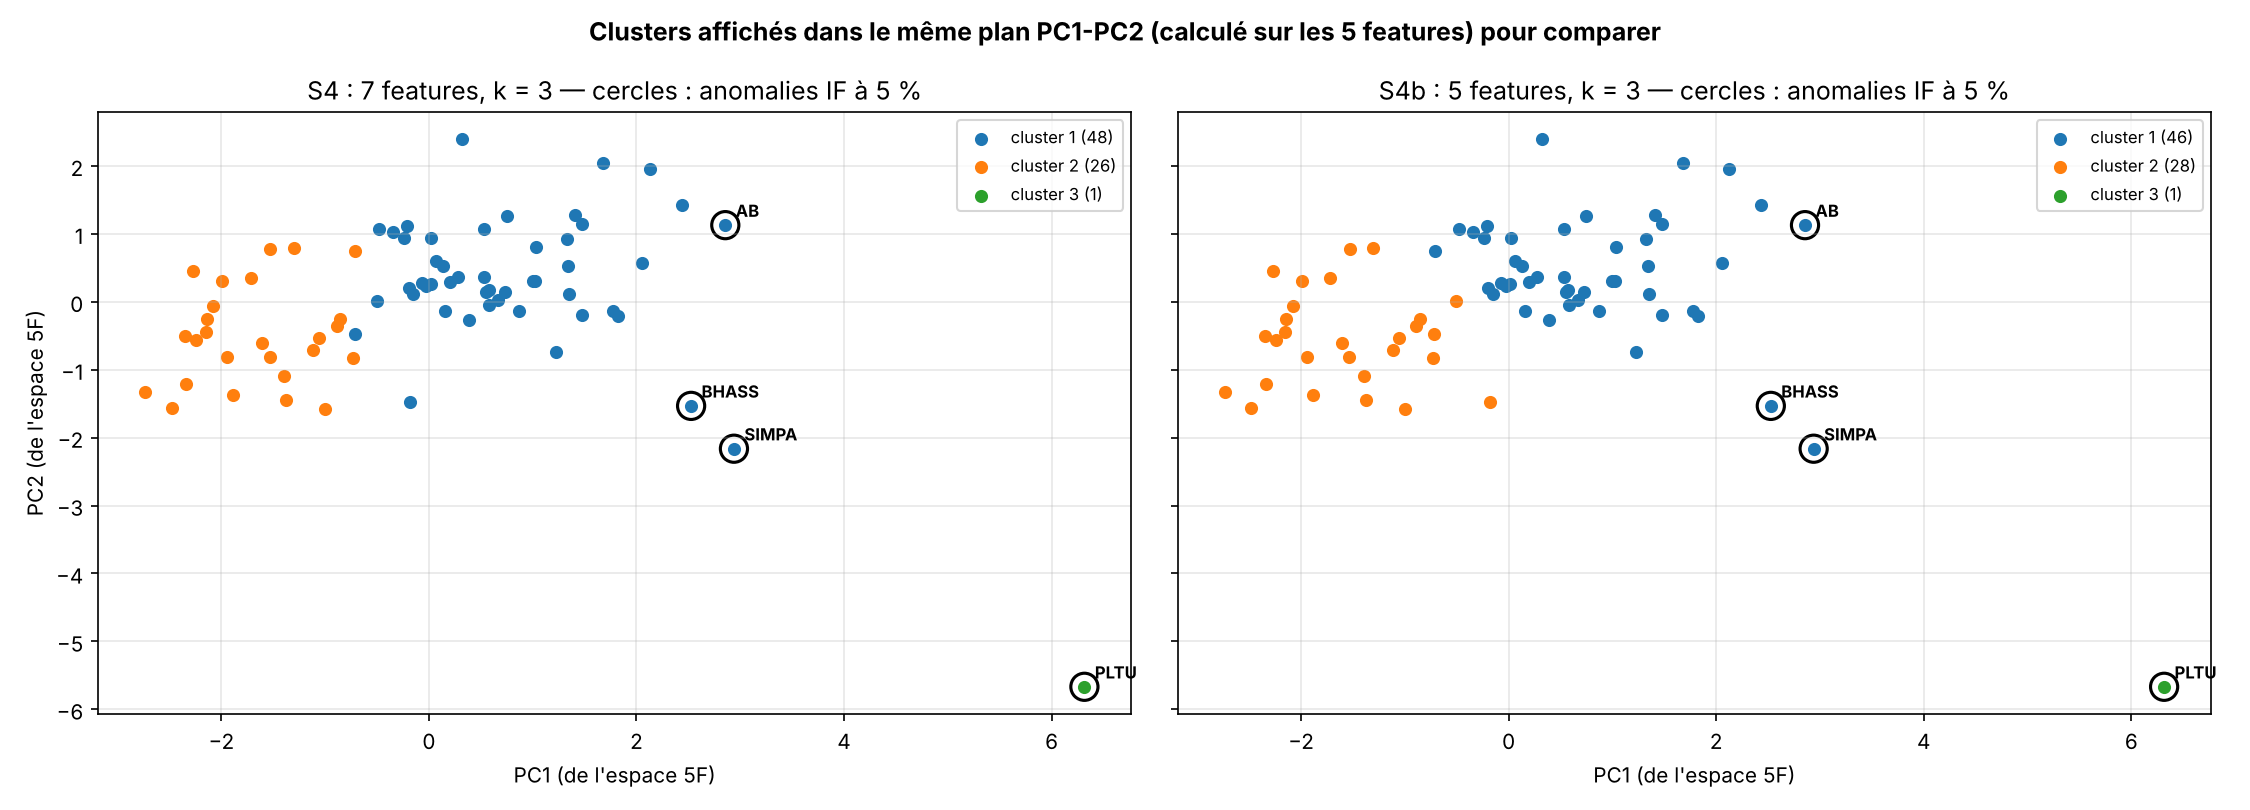
\includegraphics[width=\linewidth]{s4b_clusters_7F_vs_5F.png}
\caption{Groupes avec 7 features (S4) et avec 5 features (S4b), dans le même plan PC1-PC2 ; cercles : anomalies à 5\pc{}.}\label{fig:7f-5f}
\end{figure}

\paragraph{Sur les 57 titres liquides.} Le vote retient encore $k = 3$ (24 / 18 / 15 titres), mais la silhouette est basse (0,29) et $k = 2$ ferait mieux (0,36) : chez les titres liquides, la structure de groupes est très faible. Les anomalies stables sont AB, CELL et SOTET, toutes liquides et expliquées par une feature mesurable (AB : skewness à $+3{,}0\sigma$ ; CELL : rendement à $-2{,}2\sigma$ ; SOTET : rendement à $+2{,}2\sigma$). AB et SOTET sont confirmées ; WIFAK est remplacée par CELL.

\begin{retenir}
Retirer les features redondantes ne change pas les conclusions : mêmes groupes à quatre titres près, mêmes anomalies. Les résultats de la S4 ne venaient pas de la redondance.
\end{retenir}

\section{Restitution : une interface interactive}\label{sec:interface}
Pour rendre les résultats consultables, nous avons développé une interface Streamlit (dossier \texttt{app/} du dépôt). Elle comporte sept pages : accueil, données, paramètres, Markowitz, segmentation, anomalies et fiche par titre. Elle lit les sorties des notebooks et refait les calculs avec les mêmes paramètres et la même graine. Par défaut, elle affiche les résultats du projet ; des réglages (nombre de groupes, taux de contamination, taux sans risque, titres liquides seulement) permettent d'explorer, et chaque page signale quand on s'écarte des choix du projet. Un script de contrôle vérifie que l'interface redonne les résultats des notebooks (21 contrôles, annexe~\ref{ann:controles}).

\begin{figure}[H]\centering
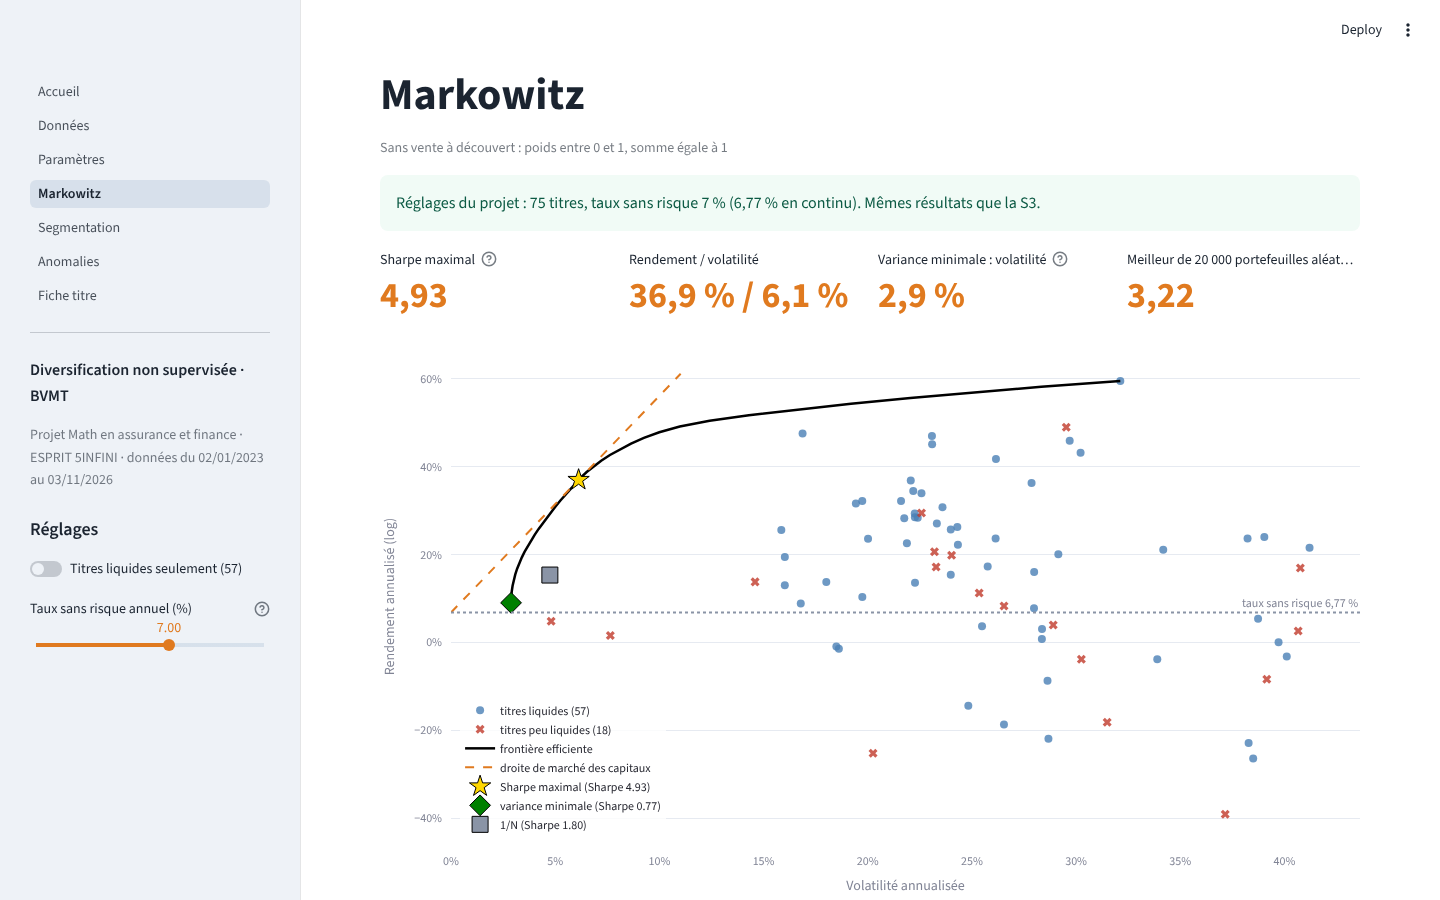
\includegraphics[width=0.85\linewidth]{interface_markowitz.png}
\caption{Page Markowitz de l'interface : frontière interactive et réglages.}\label{fig:interface}
\end{figure}

\section{Analyse critique de notre travail}\label{sec:critique}
\begin{itemize}
  \item \textbf{Tous les résultats sont dans l'échantillon.} Ni les portefeuilles de Markowitz ni les groupes n'ont encore été testés sur des données futures. C'est la limite principale, la même que celle reprochée à l'article.
  \item \textbf{La structure de groupes est faible} (silhouette de 0,29 à 0,47). Diversifier « entre groupes » n'a de sens que si les groupes sont nets ; ce point devra être vérifié par la performance des portefeuilles.
  \item \textbf{Les features restent individuelles.} Comme dans l'article, elles ne décrivent pas les co-mouvements. Une segmentation sur les corrélations entre titres serait plus proche de l'idée de diversification.
  \item \textbf{La liquidité domine.} Elle explique à la fois le premier découpage des groupes et la plupart des anomalies. Nous l'avons montré, mais pas encore corrigé dans les features (par exemple par une volatilité calculée sur les seuls jours échangés).
  \item \textbf{Biais du survivant} : les dix sociétés radiées depuis 2023 sont exclues, alors qu'elles seraient justement les anomalies les plus intéressantes à détecter.
  \item \textbf{Secteurs} : les secteurs des titres ne sont pas encore renseignés ; la comparaison entre groupes et secteurs reste à faire.
\end{itemize}

% =====================================================================
\section*{Conclusion et perspectives}
\addcontentsline{toc}{section}{Conclusion et perspectives}
% =====================================================================
L'article de Rebai et al.\ (2021) a une bonne idée, mais une preuve incomplète : il ne construit aucun portefeuille, publie des ratios de Sharpe irréalistes et ne contrôle pas la liquidité des titres qu'il juge anormaux.

Sur des données officielles 2023-2026, corrigées des opérations sur titres, nous montrons que :
\begin{enumerate}
  \item Markowitz exact reproduit les excès de l'article : un Sharpe de 4,93 dans l'échantillon, et un portefeuille de variance minimale piégé par des titres illiquides ;
  \item les groupes ne suivent pas les secteurs : ils reflètent la liquidité et la sensibilité au marché, avec une structure faible ;
  \item la plupart des anomalies sont des artefacts d'illiquidité ;
  \item ces conclusions résistent au retrait des features redondantes.
\end{enumerate}

\paragraph{Prochaines étapes.}
\begin{itemize}
  \item construire le portefeuille « un titre par groupe » et le comparer au 1/N et à Markowitz \textbf{hors échantillon} (par exemple : estimation sur 2023-2025, test sur 2026) ;
  \item lire les groupes par secteur ;
  \item justifier les anomalies liquides (SOTET, AB) avec les états financiers et les communiqués du CMF ;
  \item mettre en œuvre l'extension du projet : \afaire{extension choisie et résultats}.
\end{itemize}

% =====================================================================
\clearpage
\section*{Références}
\addcontentsline{toc}{section}{Références}
\begin{enumerate}[label={[\arabic*]},leftmargin=*]
  \item Rebai, A., Boukhris, L., Ncib, L. et Ben Lasmar, M. A. (2021). Unsupervised Learning Diversification Applied on the Tunisian Stock Market Before and During the Covid-19 Crisis. \emph{International Journal of Management Research and Economics}, 1(4), 24-47. \url{https://doi.org/10.51483/IJMRE.1.4.2021.24-47}
  \item Markowitz, H. (1952). Portfolio Selection. \emph{The Journal of Finance}, 7(1), 77-91.
  \item Sharpe, W. F. (1964). Capital Asset Prices: A Theory of Market Equilibrium under Conditions of Risk. \emph{The Journal of Finance}, 19(3), 425-442.
  \item Sharpe, W. F. (1966). Mutual Fund Performance. \emph{The Journal of Business}, 39(1), 119-138.
  \item Cornuéjols, G. et Tütüncü, R. (2007). \emph{Optimization Methods in Finance}. Cambridge University Press.
  \item DeMiguel, V., Garlappi, L. et Uppal, R. (2009). Optimal Versus Naive Diversification: How Inefficient is the 1/N Portfolio Strategy? \emph{The Review of Financial Studies}, 22(5), 1915-1953.
  \item Artzner, P., Delbaen, F., Eber, J.-M. et Heath, D. (1999). Coherent Measures of Risk. \emph{Mathematical Finance}, 9(3), 203-228.
  \item Arthur, D. et Vassilvitskii, S. (2007). k-means++: The Advantages of Careful Seeding. \emph{Proceedings of the 18th ACM-SIAM Symposium on Discrete Algorithms}, 1027-1035.
  \item Rousseeuw, P. J. (1987). Silhouettes: A Graphical Aid to the Interpretation and Validation of Cluster Analysis. \emph{Journal of Computational and Applied Mathematics}, 20, 53-65.
  \item Caliński, T. et Harabasz, J. (1974). A Dendrite Method for Cluster Analysis. \emph{Communications in Statistics}, 3(1), 1-27.
  \item Davies, D. L. et Bouldin, D. W. (1979). A Cluster Separation Measure. \emph{IEEE Transactions on Pattern Analysis and Machine Intelligence}, 1(2), 224-227.
  \item Liu, F. T., Ting, K. M. et Zhou, Z.-H. (2008). Isolation Forest. \emph{Proceedings of the 8th IEEE International Conference on Data Mining}, 413-422.
  \item Hubert, L. et Arabie, P. (1985). Comparing Partitions. \emph{Journal of Classification}, 2(1), 193-218.
  \item Bourse des valeurs mobilières de Tunis : archives de cotation et bulletins officiels de la cote, 2023-2026.
\end{enumerate}

% =====================================================================
\clearpage
\appendix
\renewcommand{\thesection}{\Alph{section}}
\section*{Annexes}
\addcontentsline{toc}{section}{Annexes}
% =====================================================================

\section{Déclaration d'usage de l'IA générative}\label{ann:ia}
Conformément au cahier des charges, nous déclarons avoir utilisé un assistant d'IA générative (Claude, Anthropic) pendant le projet, pour :
\begin{itemize}
  \item l'aide à l'écriture du code : scripts de collecte et d'extraction des bulletins PDF, notebooks S3, S4 et S4b, interface Streamlit ;
  \item l'aide à la rédaction : reformulation de textes, structure du rapport et de la présentation, code \LaTeX{} du rapport ;
  \item l'explication de notions (construction de la frontière efficiente, critères de choix de $k$).
\end{itemize}
Les choix de méthode ont été discutés et validés par l'équipe. Chaque résultat a été vérifié par des contrôles automatiques (annexe~\ref{ann:controles}) et peut être reproduit à partir du dépôt. L'équipe reste responsable de chaque ligne rendue et est en mesure de l'expliquer. \afaire{préciser, si besoin, la part de chaque membre et les vérifications faites}

\section{Reproductibilité}\label{ann:repro}
\subsection*{Dépôt et structure}
Le code est disponible sur \url{https://github.com/nadhmi54/diversification-bvmt}. Les données brutes ne sont pas versionnées (elles se retéléchargent depuis les sources officielles) ; les données traitées et toutes les sorties le sont.

\begin{verbatim}
src/                  collecte, extraction des bulletins, construction des données (S2)
notebooks/            S3_features_markowitz, S4_segmentation_anomalies,
                      S4b_segmentation_5_features, S3_S4_complet (les trois réunis)
data/processed/       données de la S2 ; sorties S4 (s4/) et S4b (s4_5f/)
data/s3/              sorties de la S3
app/                  interface Streamlit
reports/              note qualité, rapport S3, présentation
\end{verbatim}

\subsection*{Commandes}
\begin{verbatim}
pip install -r requirements.txt
python src/collecte.py
python src/parse_bulletins.py data/raw/bulletins/pdf
python src/parse_tunindex_bulletins.py
python src/build_dataset.py
jupyter nbconvert --to notebook --execute --inplace notebooks/S3_S4_complet.ipynb
streamlit run app/Accueil.py
python app/verifier_coherence.py
\end{verbatim}

\subsection*{Paramètres fixes}
Graine aléatoire 42 (k-means, Isolation Forest, ACP) ; graine 0 pour les 20\,000 portefeuilles aléatoires de contrôle ; 252 séances par an ; seuil de liquidité 60\pc{} ; taux sans risque $\ln(1{,}07)$ ; chemins relatifs dans tous les notebooks.

\section{Contrôles automatiques}\label{ann:controles}
\begin{itemize}
  \item \textbf{S3} : rendements $959 \times 75$ sans valeur manquante ; dates du Tunindex identiques à celles des titres ; VaR $\leq 0$ et CVaR $\leq$ VaR ; corrélations symétriques de diagonale 1 ; covariance définie positive ; poids de somme 1 et dans $[0,1]$ ; frontière croissante.
  \item \textbf{S4 et S4b} : 75 titres $\times$ 7 (ou 5) features sans valeur manquante ; standardisation correcte ; seuil par rang identique à \texttt{IsolationForest(contamination=taux)} pour chaque combinaison ; $k$ retenu dans la plage ; chaque titre a un groupe.
  \item \textbf{Notebook réuni} : les 33 fichiers de résultats produits par \texttt{S3\_S4\_complet} sont identiques à ceux des trois notebooks séparés.
  \item \textbf{Interface} : 21 contrôles (k retenus, groupes, scores Isolation Forest et signalements identiques à la S4 et à la S4b ; Sharpe 4,93, poids et meilleur portefeuille aléatoire identiques à la S3).
\end{itemize}

\section{Opérations sur titres}\label{ann:ost}
\begin{table}[H]\centering\small\caption{Opérations sur titres détectées par le cours de référence officiel, par type et par année}\label{tab:annexe-ost}
\begin{tabular}{lrrrrr}\toprule
Type & 2023 & 2024 & 2025 & 2026 & Total \\ \midrule
ajustement à la hausse (reprise de cotation ?) & 4 & 0 & 2 & 0 & 6 \\
attribution gratuite & 2 & 4 & 3 & 0 & 9 \\
dividende & 1 & 1 & 50 & 53 & 105 \\
dividende probable & 51 & 47 & 1 & 5 & 104 \\
division / attribution probable & 1 & 0 & 2 & 1 & 4 \\
\midrule
Total & 59 & 52 & 58 & 59 & 228 \\
\bottomrule\end{tabular}\end{table}
\begin{table}[H]\centering\small\caption{Exemple : les 5 opérations sur titres de BIAT}\label{tab:annexe-biat}
\begin{tabular}{llrrrp{5cm}}\toprule
Date & Type & Clôture veille & Référence & Facteur & Détail \\ \midrule
15/05/2023 & dividende probable & 96{,}00 & 90{,}20 & 0{,}9396 & écart 5.800 DT (6.0\%) \\
13/05/2024 & dividende probable & 95{,}80 & 89{,}80 & 0{,}9374 & écart 6.000 DT (6.3\%) \\
29/11/2024 & attribution gratuite & 105{,}00 & 91{,}88 & 0{,}8750 & BIAT DA1/7 291124 : 1 nouvelle(s) pour 7 anciennes (f théorique 0.8750) \\
12/05/2025 & dividende & 103{,}45 & 97{,}45 & 0{,}9420 & dividende 6.000 DT (bulletin) \\
12/05/2026 & dividende & 160{,}00 & 154{,}00 & 0{,}9625 & dividende 6.000 DT (bulletin) \\
\bottomrule\end{tabular}\end{table}

\section{Titres retirés de l'univers}\label{ann:retires}
\begin{table}[H]\centering\small
\caption{Les 10 sociétés présentes dans les sources mais plus cotées au 03/11/2026}\label{tab:retires}
\begin{tabular}{lll}\toprule
Société & ISIN & Dernière séance \\ \midrule
ADWYA & TN0007250012 & 05/01/2023 \\
CEREALIS & TN0007640014 & 13/02/2023 \\
AMS & TN0001500859 & 15/09/2023 \\
SOPAT & TN0007290018 & 03/11/2023 \\
SERVICOM & TN0007340011 & 30/04/2024 \\
ELECTROSTAR & TN0006650014 & 10/09/2024 \\
Maghreb International Publicité & TN0007660012 & 10/09/2024 \\
GIF-Filter & TN0007130016 & 11/11/2024 \\
Société tunisienne du sucre & TN0006170013 & 31/12/2025 \\
SITEX & TN0004300307 & 31/12/2025 \\
\bottomrule\end{tabular}
\end{table}

\section{Liste des 75 titres et résultats par titre}\label{ann:titres}
Colonnes RV, 7F, ACP, 5F : numéro du groupe k-means dans chaque espace (1 = le plus grand). IF/12 : nombre de signalements Isolation Forest sur les 12 tests de la S4.
{\small\begin{longtable}{llrrcccccc}
\caption{Les 75 titres : liquidité, groupes k-means et signalements Isolation Forest}\label{tab:annexe-titres}\\
\toprule Ticker & Nom & Séances & Rdts nuls & Liq. & RV & 7F & ACP & 5F & IF/12 \\ \midrule \endfirsthead
\toprule Ticker & Nom & Séances & Rdts nuls & Liq. & RV & 7F & ACP & 5F & IF/12 \\ \midrule \endhead \bottomrule \endfoot
AB & AMEN BANK & 99~\% & 17~\% & oui & 1 & 1 & 1 & 1 & 6 \\
AETEC & AETECH & 23~\% & 70~\% & non & 6 & 2 & 2 & 2 & 0 \\
AL & AIR LIQUIDE TSIE & 69~\% & 53~\% & oui & 1 & 1 & 1 & 1 & 0 \\
ALKIM & ALKIMIA & 18~\% & 86~\% & non & 6 & 2 & 2 & 2 & 6 \\
AMV & ASSU MAGHREBIA VIE & 93~\% & 33~\% & oui & 1 & 1 & 1 & 1 & 0 \\
ARTES & ARTES & 98~\% & 22~\% & oui & 1 & 1 & 1 & 1 & 0 \\
ASSAD & ASSAD & 88~\% & 28~\% & oui & 3 & 2 & 2 & 2 & 0 \\
ASSMA & ASSUR MAGHREBIA & 59~\% & 62~\% & non & 1 & 1 & 1 & 1 & 0 \\
AST & ASTREE & 32~\% & 79~\% & non & 2 & 1 & 2 & 2 & 0 \\
ATB & ATB & 96~\% & 25~\% & oui & 2 & 1 & 1 & 1 & 0 \\
ATL & ATL & 94~\% & 31~\% & oui & 5 & 1 & 1 & 1 & 0 \\
BH & BH BANK & 89~\% & 30~\% & oui & 2 & 1 & 1 & 1 & 0 \\
BHASS & BH ASSURANCE & 10~\% & 94~\% & non & 4 & 1 & 1 & 1 & 7 \\
BHL & BH LEASING & 69~\% & 42~\% & oui & 3 & 2 & 2 & 2 & 1 \\
BIAT & BIAT & 100~\% & 14~\% & oui & 4 & 1 & 1 & 1 & 1 \\
BL & BEST LEASE & 39~\% & 72~\% & non & 2 & 2 & 2 & 2 & 0 \\
BNA & BNA & 100~\% & 18~\% & oui & 1 & 1 & 1 & 1 & 0 \\
BNASS & BNA ASSURANCES & 90~\% & 25~\% & oui & 2 & 1 & 1 & 1 & 0 \\
BT & BT & 100~\% & 30~\% & oui & 4 & 1 & 1 & 1 & 0 \\
BTE & BTE (ADP) & 69~\% & 40~\% & oui & 3 & 2 & 2 & 2 & 0 \\
CC & CARTHAGE CEMENT & 100~\% & 24~\% & oui & 4 & 1 & 1 & 1 & 0 \\
CELL & CELLCOM & 69~\% & 35~\% & oui & 7 & 2 & 2 & 2 & 2 \\
CIL & CIL & 79~\% & 44~\% & oui & 5 & 1 & 1 & 1 & 0 \\
CITY & CITY CARS & 98~\% & 22~\% & oui & 1 & 1 & 1 & 1 & 0 \\
DH & DELICE HOLDING & 99~\% & 19~\% & oui & 1 & 1 & 1 & 1 & 0 \\
ECYCL & EURO-CYCLES & 100~\% & 11~\% & oui & 6 & 2 & 2 & 2 & 0 \\
HL & HANNIBAL LEASE & 56~\% & 69~\% & non & 1 & 1 & 1 & 1 & 0 \\
ICF & ICF & 96~\% & 16~\% & oui & 2 & 1 & 1 & 2 & 0 \\
LNDOR & LAND OR & 95~\% & 21~\% & oui & 1 & 1 & 1 & 1 & 0 \\
MAG & MAGASIN GENERAL & 48~\% & 65~\% & non & 2 & 2 & 2 & 2 & 0 \\
MGR & SOTUMAG & 94~\% & 32~\% & oui & 5 & 1 & 1 & 1 & 0 \\
MNP & MONOPRIX & 71~\% & 46~\% & oui & 3 & 2 & 2 & 2 & 0 \\
MPBS & MPBS & 92~\% & 29~\% & oui & 5 & 1 & 1 & 1 & 0 \\
NAKL & ENNAKL AUTOMOBILES & 86~\% & 33~\% & oui & 2 & 1 & 1 & 1 & 0 \\
NBL & NEW BODY LINE & 84~\% & 39~\% & oui & 6 & 2 & 2 & 2 & 0 \\
OTH & ONE TECH HOLDING & 99~\% & 15~\% & oui & 4 & 1 & 1 & 1 & 0 \\
PGH & POULINA GP HOLDING & 97~\% & 20~\% & oui & 1 & 1 & 1 & 1 & 0 \\
PLAST & OFFICEPLAST & 75~\% & 38~\% & oui & 3 & 2 & 2 & 2 & 0 \\
PLTU & PLAC. TSIE-SICAF & 4~\% & 98~\% & non & 8 & 3 & 3 & 3 & 12 \\
SAH & SAH & 100~\% & 18~\% & oui & 4 & 1 & 1 & 1 & 0 \\
SAM & ATELIER MEUBLE INT & 99~\% & 28~\% & oui & 1 & 1 & 1 & 1 & 0 \\
SCB & CIMENTS DE BIZERTE & 65~\% & 44~\% & oui & 7 & 2 & 2 & 2 & 1 \\
SFBT & SFBT & 100~\% & 19~\% & oui & 4 & 1 & 1 & 1 & 0 \\
SIAME & SIAME & 95~\% & 26~\% & oui & 2 & 2 & 2 & 2 & 0 \\
SIMPA & SIMPAR & 12~\% & 97~\% & non & 8 & 1 & 1 & 1 & 11 \\
SIPHA & SIPHAT & 34~\% & 69~\% & non & 6 & 2 & 2 & 2 & 0 \\
SITS & SITS & 25~\% & 80~\% & non & 2 & 2 & 2 & 2 & 0 \\
SMART & SMART TUNISIE & 96~\% & 22~\% & oui & 1 & 1 & 1 & 1 & 0 \\
SMD & SANIMED & 27~\% & 58~\% & non & 7 & 2 & 2 & 2 & 5 \\
SOKNA & ESSOUKNA & 75~\% & 35~\% & oui & 3 & 2 & 2 & 2 & 0 \\
SOMOC & SOMOCER & 92~\% & 44~\% & oui & 3 & 2 & 2 & 2 & 0 \\
SOTEM & SOTEMAIL & 10~\% & 64~\% & non & 3 & 2 & 2 & 2 & 0 \\
SOTET & SOTETEL & 99~\% & 16~\% & oui & 5 & 1 & 1 & 1 & 10 \\
SOTUV & SOTUVER & 99~\% & 16~\% & oui & 1 & 1 & 1 & 1 & 0 \\
SPDIT & SPDIT - SICAF & 87~\% & 48~\% & oui & 1 & 1 & 1 & 1 & 0 \\
STA & STA & 87~\% & 27~\% & oui & 5 & 1 & 1 & 1 & 0 \\
STAR & STAR & 72~\% & 47~\% & oui & 1 & 1 & 1 & 1 & 0 \\
STB & STB & 99~\% & 23~\% & oui & 2 & 1 & 1 & 1 & 0 \\
STIP & STIP & 49~\% & 54~\% & non & 3 & 2 & 2 & 2 & 0 \\
STPAP & SOTIPAPIER & 97~\% & 23~\% & oui & 6 & 2 & 2 & 2 & 0 \\
STPIL & SOTRAPIL & 94~\% & 24~\% & oui & 1 & 1 & 1 & 1 & 0 \\
TAIR & TUNISAIR & 90~\% & 56~\% & oui & 6 & 2 & 2 & 2 & 1 \\
TGH & TAWASOL GP HOLDING & 89~\% & 32~\% & oui & 3 & 2 & 2 & 2 & 0 \\
TINV & TUNINVEST-SICAR & 43~\% & 63~\% & non & 5 & 2 & 2 & 1 & 0 \\
TJARI & ATTIJARI BANK & 100~\% & 12~\% & oui & 1 & 1 & 1 & 1 & 0 \\
TJL & ATTIJARI LEASING & 79~\% & 45~\% & oui & 1 & 1 & 1 & 1 & 0 \\
TLNET & TELNET HOLDING & 99~\% & 16~\% & oui & 2 & 1 & 1 & 1 & 0 \\
TLS & TUNISIE LEASING F & 86~\% & 30~\% & oui & 5 & 1 & 1 & 1 & 0 \\
TPR & TPR & 100~\% & 16~\% & oui & 1 & 1 & 1 & 1 & 0 \\
TRE & TUNIS RE & 81~\% & 46~\% & oui & 1 & 1 & 1 & 1 & 0 \\
UADH & UADH & 51~\% & 41~\% & non & 3 & 2 & 2 & 2 & 0 \\
UBCI & UBCI & 47~\% & 69~\% & non & 1 & 1 & 1 & 1 & 0 \\
UIB & UIB & 94~\% & 27~\% & oui & 2 & 1 & 1 & 1 & 0 \\
UMED & UNIMED & 99~\% & 18~\% & oui & 4 & 1 & 1 & 1 & 0 \\
WIFAK & WIFACK INT BANK & 69~\% & 61~\% & oui & 4 & 1 & 1 & 2 & 0 \\
\end{longtable}}

\section{Features des 75 titres}\label{ann:features}
{\small\begin{longtable}{lrrrrrrr}
\caption{Les 7 features des 75 titres (rendement et volatilité annualisés ; VaR et CVaR journalières à 95~\%)}\label{tab:annexe-features}\\
\toprule Ticker & Rendement & Volatilité & Skewness & Kurtosis & VaR & CVaR & Bêta \\ \midrule \endfirsthead
\toprule Ticker & Rendement & Volatilité & Skewness & Kurtosis & VaR & CVaR & Bêta \\ \midrule \endhead \bottomrule \endfoot
AB & 47{,}5~\% & 16{,}9~\% & 1{,}48 & 5{,}36 & $-$1{,}12~\% & $-$1{,}74~\% & 1{,}02 \\
AETEC & $-$18{,}2~\% & 31{,}5~\% & $-$0{,}03 & 0{,}95 & $-$3{,}92~\% & $-$4{,}36~\% & $-$0{,}05 \\
AL & 31{,}6~\% & 19{,}4~\% & 0{,}09 & 5{,}31 & $-$1{,}70~\% & $-$3{,}20~\% & $-$0{,}02 \\
ALKIM & $-$25{,}2~\% & 20{,}3~\% & $-$0{,}78 & 8{,}20 & $-$3{,}29~\% & $-$4{,}41~\% & 0{,}01 \\
AMV & 23{,}6~\% & 20{,}0~\% & 0{,}98 & 4{,}89 & $-$1{,}75~\% & $-$2{,}58~\% & 0{,}62 \\
ARTES & 26{,}2~\% & 24{,}3~\% & 0{,}56 & 3{,}73 & $-$1{,}99~\% & $-$3{,}21~\% & 0{,}52 \\
ASSAD & 23{,}9~\% & 39{,}0~\% & 0{,}06 & $-$0{,}46 & $-$4{,}31~\% & $-$4{,}50~\% & 0{,}14 \\
ASSMA & 19{,}8~\% & 24{,}0~\% & 0{,}39 & 4{,}43 & $-$2{,}29~\% & $-$3{,}88~\% & 0{,}47 \\
AST & 17{,}1~\% & 23{,}3~\% & 0{,}03 & 5{,}30 & $-$2{,}26~\% & $-$4{,}27~\% & $-$0{,}05 \\
ATB & 3{,}7~\% & 25{,}5~\% & 0{,}05 & 2{,}17 & $-$2{,}54~\% & $-$3{,}76~\% & 0{,}68 \\
ATL & 46{,}9~\% & 23{,}1~\% & 0{,}83 & 3{,}69 & $-$1{,}90~\% & $-$2{,}88~\% & 0{,}80 \\
BH & 3{,}0~\% & 28{,}4~\% & 0{,}22 & 2{,}37 & $-$2{,}93~\% & $-$4{,}20~\% & 1{,}11 \\
BHASS & 13{,}7~\% & 14{,}6~\% & 1{,}02 & 18{,}92 & 0{,}00~\% & $-$0{,}08~\% & 0{,}11 \\
BHL & 21{,}5~\% & 41{,}2~\% & $-$0{,}10 & $-$0{,}03 & $-$4{,}50~\% & $-$5{,}09~\% & 0{,}14 \\
BIAT & 25{,}5~\% & 15{,}9~\% & 0{,}54 & 6{,}36 & $-$1{,}19~\% & $-$2{,}14~\% & 1{,}41 \\
BL & 8{,}3~\% & 26{,}5~\% & 0{,}02 & 2{,}80 & $-$4{,}15~\% & $-$4{,}35~\% & 0{,}03 \\
BNA & 30{,}7~\% & 23{,}6~\% & 0{,}69 & 3{,}85 & $-$1{,}95~\% & $-$2{,}96~\% & 1{,}56 \\
BNASS & 20{,}0~\% & 29{,}1~\% & 0{,}20 & 0{,}20 & $-$2{,}88~\% & $-$3{,}27~\% & 0{,}66 \\
BT & 19{,}4~\% & 16{,}0~\% & 0{,}65 & 6{,}15 & $-$1{,}32~\% & $-$2{,}12~\% & 1{,}01 \\
BTE & $-$3{,}3~\% & 40{,}1~\% & $-$0{,}10 & $-$0{,}33 & $-$4{,}52~\% & $-$4{,}55~\% & 0{,}36 \\
CC & $-$1{,}0~\% & 18{,}5~\% & 0{,}79 & 2{,}57 & $-$1{,}58~\% & $-$2{,}19~\% & 0{,}58 \\
CELL & $-$22{,}9~\% & 38{,}3~\% & $-$0{,}13 & $-$0{,}20 & $-$4{,}41~\% & $-$4{,}81~\% & $-$0{,}08 \\
CIL & 36{,}2~\% & 27{,}9~\% & 0{,}13 & 1{,}85 & $-$3{,}18~\% & $-$4{,}22~\% & 0{,}56 \\
CITY & 22{,}6~\% & 21{,}9~\% & 0{,}52 & 3{,}82 & $-$2{,}04~\% & $-$3{,}00~\% & 0{,}42 \\
DH & 32{,}1~\% & 21{,}6~\% & 0{,}54 & 2{,}79 & $-$1{,}95~\% & $-$2{,}73~\% & 0{,}84 \\
ECYCL & $-$18{,}7~\% & 26{,}5~\% & 0{,}30 & 2{,}65 & $-$2{,}55~\% & $-$3{,}87~\% & 0{,}49 \\
HL & 29{,}4~\% & 22{,}6~\% & 0{,}03 & 4{,}74 & $-$1{,}98~\% & $-$3{,}93~\% & 0{,}24 \\
ICF & 16{,}0~\% & 28{,}0~\% & 0{,}33 & 2{,}83 & $-$2{,}59~\% & $-$3{,}95~\% & 0{,}32 \\
LNDOR & 23{,}6~\% & 26{,}1~\% & 0{,}39 & 3{,}14 & $-$2{,}39~\% & $-$3{,}62~\% & 0{,}57 \\
MAG & 3{,}9~\% & 28{,}9~\% & $-$0{,}05 & 2{,}22 & $-$4{,}45~\% & $-$4{,}54~\% & $-$0{,}12 \\
MGR & 45{,}1~\% & 23{,}1~\% & 1{,}01 & 4{,}02 & $-$2{,}01~\% & $-$2{,}82~\% & 0{,}26 \\
MNP & 21{,}1~\% & 34{,}2~\% & $-$0{,}06 & 0{,}88 & $-$4{,}40~\% & $-$4{,}76~\% & 0{,}48 \\
MPBS & 43{,}1~\% & 30{,}2~\% & 0{,}40 & 2{,}34 & $-$2{,}77~\% & $-$4{,}23~\% & 0{,}40 \\
NAKL & 15{,}3~\% & 24{,}0~\% & 0{,}50 & 4{,}13 & $-$2{,}16~\% & $-$3{,}42~\% & 0{,}38 \\
NBL & $-$14{,}5~\% & 24{,}8~\% & $-$0{,}31 & 4{,}39 & $-$2{,}61~\% & $-$4{,}34~\% & 0{,}32 \\
OTH & 13{,}7~\% & 18{,}0~\% & 0{,}77 & 3{,}77 & $-$1{,}56~\% & $-$2{,}25~\% & 0{,}63 \\
PGH & 33{,}9~\% & 22{,}6~\% & 0{,}61 & 3{,}64 & $-$1{,}97~\% & $-$3{,}03~\% & 0{,}70 \\
PLAST & 0{,}0~\% & 39{,}7~\% & $-$0{,}08 & $-$0{,}37 & $-$4{,}37~\% & $-$4{,}66~\% & 0{,}01 \\
PLTU & 4{,}8~\% & 4{,}8~\% & 11{,}73 & 164{,}31 & 0{,}00~\% & $-$0{,}00~\% & $-$0{,}00 \\
SAH & 13{,}0~\% & 16{,}0~\% & 0{,}74 & 3{,}61 & $-$1{,}40~\% & $-$1{,}91~\% & 0{,}69 \\
SAM & 29{,}3~\% & 22{,}3~\% & 0{,}57 & 3{,}80 & $-$1{,}91~\% & $-$2{,}98~\% & 0{,}37 \\
SCB & $-$26{,}4~\% & 38{,}5~\% & $-$0{,}02 & $-$0{,}65 & $-$4{,}17~\% & $-$4{,}32~\% & 0{,}14 \\
SFBT & 8{,}8~\% & 16{,}8~\% & 0{,}97 & 4{,}87 & $-$1{,}46~\% & $-$2{,}14~\% & 0{,}82 \\
SIAME & 0{,}7~\% & 28{,}4~\% & 0{,}18 & 2{,}70 & $-$2{,}90~\% & $-$4{,}18~\% & 0{,}40 \\
SIMPA & 1{,}5~\% & 7{,}6~\% & 1{,}28 & 68{,}76 & 0{,}00~\% & $-$0{,}03~\% & 0{,}08 \\
SIPHA & $-$3{,}8~\% & 30{,}3~\% & $-$0{,}22 & 1{,}90 & $-$4{,}47~\% & $-$4{,}54~\% & 0{,}11 \\
SITS & 11{,}2~\% & 25{,}3~\% & 0{,}02 & 3{,}83 & $-$4{,}12~\% & $-$4{,}39~\% & 0{,}11 \\
SMART & 25{,}7~\% & 24{,}0~\% & 0{,}85 & 2{,}73 & $-$2{,}06~\% & $-$3{,}05~\% & 0{,}35 \\
SMD & $-$39{,}1~\% & 37{,}2~\% & $-$0{,}06 & $-$0{,}24 & $-$4{,}30~\% & $-$4{,}44~\% & 0{,}16 \\
SOKNA & 23{,}6~\% & 38{,}2~\% & $-$0{,}04 & $-$0{,}15 & $-$4{,}26~\% & $-$4{,}59~\% & 0{,}40 \\
SOMOC & $-$3{,}9~\% & 33{,}9~\% & $-$0{,}07 & 0{,}05 & $-$4{,}08~\% & $-$4{,}54~\% & $-$0{,}02 \\
SOTEM & $-$8{,}4~\% & 39{,}2~\% & $-$0{,}09 & $-$0{,}03 & $-$4{,}46~\% & $-$4{,}53~\% & 0{,}16 \\
SOTET & 59{,}4~\% & 32{,}1~\% & 0{,}42 & 1{,}36 & $-$2{,}79~\% & $-$4{,}03~\% & 0{,}95 \\
SOTUV & 28{,}2~\% & 21{,}8~\% & 0{,}91 & 4{,}93 & $-$1{,}68~\% & $-$2{,}64~\% & 0{,}75 \\
SPDIT & 28{,}3~\% & 22{,}4~\% & 0{,}13 & 3{,}88 & $-$2{,}23~\% & $-$3{,}61~\% & 0{,}32 \\
STA & 45{,}9~\% & 29{,}7~\% & 0{,}20 & 2{,}82 & $-$2{,}60~\% & $-$4{,}40~\% & 0{,}32 \\
STAR & 28{,}5~\% & 22{,}3~\% & 0{,}15 & 4{,}52 & $-$1{,}80~\% & $-$3{,}56~\% & 0{,}94 \\
STB & 7{,}7~\% & 28{,}0~\% & 0{,}37 & 2{,}56 & $-$2{,}70~\% & $-$3{,}94~\% & 1{,}08 \\
STIP & 16{,}9~\% & 40{,}8~\% & $-$0{,}09 & $-$0{,}25 & $-$4{,}54~\% & $-$4{,}58~\% & 0{,}20 \\
STPAP & $-$21{,}9~\% & 28{,}7~\% & 0{,}13 & 2{,}28 & $-$3{,}01~\% & $-$4{,}31~\% & 0{,}27 \\
STPIL & 27{,}0~\% & 23{,}3~\% & 0{,}58 & 3{,}64 & $-$2{,}02~\% & $-$3{,}12~\% & 0{,}41 \\
TAIR & $-$8{,}7~\% & 28{,}6~\% & 0{,}00 & $-$0{,}53 & $-$2{,}90~\% & $-$3{,}14~\% & $-$0{,}19 \\
TGH & 5{,}4~\% & 38{,}7~\% & $-$0{,}04 & $-$0{,}57 & $-$4{,}09~\% & $-$4{,}69~\% & 0{,}09 \\
TINV & 48{,}9~\% & 29{,}5~\% & 0{,}15 & 1{,}81 & $-$4{,}05~\% & $-$4{,}48~\% & 0{,}04 \\
TJARI & 32{,}1~\% & 19{,}7~\% & 0{,}54 & 3{,}96 & $-$1{,}60~\% & $-$2{,}56~\% & 1{,}53 \\
TJL & 36{,}8~\% & 22{,}1~\% & 0{,}82 & 4{,}68 & $-$2{,}01~\% & $-$2{,}89~\% & 0{,}40 \\
TLNET & 17{,}2~\% & 25{,}8~\% & 0{,}53 & 2{,}99 & $-$2{,}24~\% & $-$3{,}43~\% & 0{,}65 \\
TLS & 41{,}7~\% & 26{,}2~\% & 0{,}45 & 2{,}27 & $-$2{,}40~\% & $-$3{,}44~\% & 0{,}60 \\
TPR & 34{,}4~\% & 22{,}2~\% & 0{,}64 & 2{,}76 & $-$1{,}88~\% & $-$2{,}67~\% & 0{,}95 \\
TRE & 22{,}2~\% & 24{,}3~\% & 0{,}16 & 2{,}70 & $-$2{,}53~\% & $-$3{,}81~\% & 0{,}29 \\
UADH & 2{,}6~\% & 40{,}7~\% & $-$0{,}05 & $-$0{,}95 & $-$4{,}01~\% & $-$4{,}29~\% & 0{,}04 \\
UBCI & 20{,}6~\% & 23{,}2~\% & 0{,}26 & 4{,}68 & $-$2{,}21~\% & $-$3{,}93~\% & 0{,}41 \\
UIB & 13{,}5~\% & 22{,}3~\% & 0{,}35 & 3{,}61 & $-$1{,}98~\% & $-$3{,}15~\% & 0{,}62 \\
UMED & 10{,}3~\% & 19{,}7~\% & 0{,}35 & 4{,}08 & $-$1{,}82~\% & $-$2{,}74~\% & 0{,}58 \\
WIFAK & $-$1{,}5~\% & 18{,}6~\% & 0{,}04 & 7{,}36 & $-$1{,}97~\% & $-$3{,}24~\% & $-$0{,}15 \\
\end{longtable}}

\section{Critères de choix de \texorpdfstring{$k$}{k}}\label{ann:criteres}
\begin{table}[H]\centering\small
\caption{Critères de choix de $k$, 75 titres (S4)}\label{tab:annexe-k75}
\begin{tabular}{llrrrrl}\toprule
Espace & $k$ & Inertie & Silhouette & CH & DB & Tailles \\ \midrule
RV & 3 & 58{,}0 & 0{,}407 & 57{,}2 & 0{,}820 & 37 / 26 / 12 \\
RV & 4 & 42{,}5 & 0{,}421 & 59{,}8 & 0{,}839 & 37 / 17 / 11 / 10 \\
RV & 5 & 32{,}7 & 0{,}383 & 62{,}8 & 0{,}802 & 26 / 17 / 11 / 11 / 10 \\
RV & 6 & 26{,}0 & 0{,}401 & 65{,}8 & 0{,}734 & 22 / 13 / 11 / 11 / 10 / 8 \\
RV & 7 & 21{,}0 & 0{,}413 & 69{,}5 & 0{,}667 & 21 / 15 / 11 / 10 / 8 / 7 / 3 \\
RV & 8 & 17{,}5 & 0{,}441 & 72{,}6 & 0{,}626 & 22 / 13 / 11 / 9 / 8 / 7 / 3 / 2 \\
\midrule
7F & 3 & 203{,}3 & 0{,}406 & 57{,}0 & 0{,}657 & 48 / 26 / 1 \\
7F & 4 & 158{,}1 & 0{,}314 & 54{,}9 & 0{,}904 & 33 / 25 / 16 / 1 \\
7F & 5 & 127{,}7 & 0{,}309 & 54{,}5 & 0{,}829 & 30 / 25 / 17 / 2 / 1 \\
7F & 6 & 107{,}0 & 0{,}288 & 53{,}9 & 0{,}912 & 29 / 16 / 16 / 11 / 2 / 1 \\
7F & 7 & 94{,}6 & 0{,}274 & 51{,}6 & 0{,}922 & 25 / 16 / 15 / 10 / 6 / 2 / 1 \\
7F & 8 & 82{,}4 & 0{,}283 & 51{,}4 & 0{,}902 & 21 / 16 / 12 / 10 / 7 / 6 / 2 / 1 \\
\midrule
ACP & 3 & 148{,}2 & 0{,}469 & 77{,}4 & 0{,}550 & 47 / 27 / 1 \\
ACP & 4 & 108{,}6 & 0{,}412 & 78{,}1 & 0{,}730 & 38 / 26 / 10 / 1 \\
ACP & 5 & 85{,}2 & 0{,}370 & 78{,}4 & 0{,}702 & 32 / 23 / 17 / 2 / 1 \\
ACP & 6 & 65{,}1 & 0{,}367 & 85{,}2 & 0{,}750 & 28 / 18 / 17 / 9 / 2 / 1 \\
ACP & 7 & 53{,}1 & 0{,}373 & 88{,}3 & 0{,}708 & 27 / 17 / 14 / 8 / 6 / 2 / 1 \\
ACP & 8 & 43{,}6 & 0{,}382 & 92{,}9 & 0{,}694 & 23 / 16 / 14 / 8 / 6 / 5 / 2 / 1 \\
\bottomrule\end{tabular}\end{table}
\begin{table}[H]\centering\small
\caption{Critères de choix de $k$, 57 titres liquides (S4)}\label{tab:annexe-k57}
\begin{tabular}{llrrrrl}\toprule
Espace & $k$ & Inertie & Silhouette & CH & DB & Tailles \\ \midrule
RV & 3 & 41{,}4 & 0{,}394 & 47{,}3 & 0{,}912 & 29 / 18 / 10 \\
RV & 4 & 30{,}7 & 0{,}379 & 47{,}9 & 0{,}862 & 28 / 11 / 11 / 7 \\
RV & 5 & 23{,}8 & 0{,}406 & 49{,}4 & 0{,}839 & 23 / 11 / 9 / 7 / 7 \\
RV & 6 & 18{,}0 & 0{,}425 & 54{,}5 & 0{,}776 & 23 / 9 / 8 / 7 / 6 / 4 \\
RV & 7 & 13{,}9 & 0{,}427 & 60{,}1 & 0{,}703 & 18 / 9 / 9 / 7 / 5 / 5 / 4 \\
RV & 8 & 11{,}7 & 0{,}465 & 61{,}1 & 0{,}623 & 19 / 9 / 8 / 7 / 4 / 4 / 4 / 2 \\
\midrule
7F & 3 & 151{,}6 & 0{,}314 & 44{,}1 & 1{,}135 & 23 / 23 / 11 \\
7F & 4 & 127{,}5 & 0{,}260 & 37{,}6 & 1{,}288 & 18 / 14 / 14 / 11 \\
7F & 5 & 108{,}6 & 0{,}265 & 34{,}7 & 1{,}201 & 17 / 13 / 11 / 10 / 6 \\
7F & 6 & 96{,}1 & 0{,}280 & 32{,}1 & 1{,}130 & 16 / 11 / 10 / 10 / 8 / 2 \\
7F & 7 & 85{,}4 & 0{,}300 & 30{,}6 & 1{,}033 & 16 / 11 / 10 / 8 / 7 / 3 / 2 \\
7F & 8 & 76{,}4 & 0{,}278 & 29{,}5 & 1{,}077 & 13 / 11 / 10 / 8 / 5 / 5 / 3 / 2 \\
\midrule
ACP & 3 & 88{,}8 & 0{,}427 & 72{,}9 & 0{,}840 & 26 / 21 / 10 \\
ACP & 4 & 65{,}9 & 0{,}428 & 70{,}4 & 0{,}761 & 26 / 15 / 10 / 6 \\
ACP & 5 & 49{,}3 & 0{,}392 & 73{,}7 & 0{,}805 & 15 / 14 / 11 / 10 / 7 \\
ACP & 6 & 40{,}3 & 0{,}424 & 72{,}9 & 0{,}754 & 13 / 11 / 10 / 9 / 7 / 7 \\
ACP & 7 & 34{,}4 & 0{,}404 & 71{,}3 & 0{,}739 & 13 / 11 / 9 / 7 / 7 / 6 / 4 \\
ACP & 8 & 28{,}9 & 0{,}391 & 72{,}5 & 0{,}746 & 13 / 8 / 8 / 7 / 6 / 6 / 5 / 4 \\
\bottomrule\end{tabular}\end{table}
\begin{table}[H]\centering\small
\caption{Critères de choix de $k$, 5 features (S4b) : 75 titres et 57 liquides}\label{tab:annexe-k5f}
\begin{tabular}{llrrrrl}\toprule
Espace & $k$ & Inertie & Silhouette & CH & DB & Tailles \\ \midrule
5F & 3 & 167{,}6 & 0{,}365 & 44{,}5 & 0{,}735 & 46 / 28 / 1 \\
5F & 4 & 130{,}5 & 0{,}293 & 44{,}3 & 0{,}935 & 31 / 27 / 16 / 1 \\
5F & 5 & 109{,}8 & 0{,}296 & 42{,}3 & 0{,}835 & 28 / 24 / 20 / 2 / 1 \\
5F & 6 & 91{,}1 & 0{,}293 & 43{,}0 & 0{,}882 & 27 / 19 / 16 / 10 / 2 / 1 \\
5F & 7 & 80{,}2 & 0{,}278 & 41{,}6 & 0{,}928 & 26 / 14 / 13 / 11 / 8 / 2 / 1 \\
5F & 8 & 70{,}5 & 0{,}273 & 41{,}3 & 0{,}932 & 22 / 12 / 10 / 10 / 10 / 8 / 2 / 1 \\
\midrule
5F (57) & 3 & 117{,}2 & 0{,}286 & 38{,}6 & 1{,}185 & 24 / 18 / 15 \\
5F (57) & 4 & 99{,}8 & 0{,}278 & 32{,}8 & 1{,}167 & 22 / 18 / 10 / 7 \\
5F (57) & 5 & 85{,}8 & 0{,}233 & 30{,}2 & 1{,}225 & 14 / 13 / 13 / 10 / 7 \\
5F (57) & 6 & 76{,}3 & 0{,}269 & 27{,}9 & 1{,}068 & 18 / 15 / 10 / 6 / 5 / 3 \\
5F (57) & 7 & 67{,}3 & 0{,}284 & 26{,}9 & 1{,}071 & 15 / 11 / 10 / 8 / 7 / 3 / 3 \\
5F (57) & 8 & 58{,}3 & 0{,}278 & 27{,}2 & 1{,}051 & 13 / 10 / 8 / 7 / 6 / 5 / 5 / 3 \\
\bottomrule\end{tabular}\end{table}

\section{Stabilité des anomalies}\label{ann:stabilite}
\begin{table}[H]\centering\small
\caption{Titres signalés par Isolation Forest, 75 titres (S4)}\label{tab:annexe-if75}
\begin{tabular}{llrp{9cm}}\toprule
Espace & Taux & Signalés & Titres \\ \midrule
RV & 3\% & 3 & PLTU, SMD, SOTET \\
RV & 5\% & 4 & PLTU, SIMPA, SMD, SOTET \\
RV & 8\% & 6 & AB, ALKIM, PLTU, SIMPA, SMD, SOTET \\
RV & 10\% & 8 & AB, ALKIM, BHL, PLTU, SCB, SIMPA, SMD, SOTET \\
7F & 3\% & 3 & BHASS, PLTU, SIMPA \\
7F & 5\% & 4 & AB, BHASS, PLTU, SIMPA \\
7F & 8\% & 6 & AB, ALKIM, BHASS, PLTU, SIMPA, SOTET \\
7F & 10\% & 8 & AB, ALKIM, BHASS, BIAT, PLTU, SIMPA, SOTET, TAIR \\
ACP & 3\% & 3 & PLTU, SIMPA, SOTET \\
ACP & 5\% & 4 & BHASS, PLTU, SIMPA, SOTET \\
ACP & 8\% & 6 & ALKIM, BHASS, CELL, PLTU, SIMPA, SOTET \\
ACP & 10\% & 8 & AB, ALKIM, BHASS, CELL, PLTU, SIMPA, SMD, SOTET \\
\bottomrule\end{tabular}\end{table}
\begin{table}[H]\centering\small
\caption{Titres signalés par Isolation Forest, 57 titres liquides (S4)}\label{tab:annexe-if57}
\begin{tabular}{llrp{9cm}}\toprule
Espace & Taux & Signalés & Titres \\ \midrule
RV & 3\% & 2 & SCB, SOTET \\
RV & 5\% & 3 & BHL, SCB, SOTET \\
RV & 8\% & 5 & AB, BHL, CELL, SCB, SOTET \\
RV & 10\% & 6 & AB, BHL, BTE, CELL, SCB, SOTET \\
7F & 3\% & 2 & AB, WIFAK \\
7F & 5\% & 3 & AB, BIAT, WIFAK \\
7F & 8\% & 5 & AB, BHL, BIAT, TAIR, WIFAK \\
7F & 10\% & 6 & AB, BHL, BIAT, CELL, TAIR, WIFAK \\
ACP & 3\% & 2 & SOTET, WIFAK \\
ACP & 5\% & 3 & AB, SOTET, WIFAK \\
ACP & 8\% & 5 & AB, CELL, NBL, SOTET, WIFAK \\
ACP & 10\% & 6 & AB, BHL, CELL, NBL, SOTET, WIFAK \\
\bottomrule\end{tabular}\end{table}
\begin{table}[H]\centering\small
\caption{Titres signalés par Isolation Forest, 5 features, 75 titres (S4b)}\label{tab:annexe-if5f}
\begin{tabular}{lrp{9cm}}\toprule
Taux & Signalés & Titres \\ \midrule
3\% & 3 & AB, SIMPA, PLTU \\
5\% & 4 & AB, SIMPA, BHASS, PLTU \\
8\% & 6 & AB, SOTET, ALKIM, SIMPA, BHASS, PLTU \\
10\% & 8 & BIAT, AB, SOTET, CELL, ALKIM, SIMPA, BHASS, PLTU \\
\bottomrule\end{tabular}\end{table}
\begin{table}[H]\centering\small
\caption{Titres signalés par Isolation Forest, 5 features, 57 titres liquides (S4b)}\label{tab:annexe-if5f57}
\begin{tabular}{lrp{9cm}}\toprule
Taux & Signalés & Titres \\ \midrule
3\% & 2 & AB, CELL \\
5\% & 3 & AB, SOTET, CELL \\
8\% & 5 & AB, SOTET, NBL, BHL, CELL \\
10\% & 6 & AB, SOTET, TAIR, NBL, BHL, CELL \\
\bottomrule\end{tabular}\end{table}

\begin{figure}[H]\centering
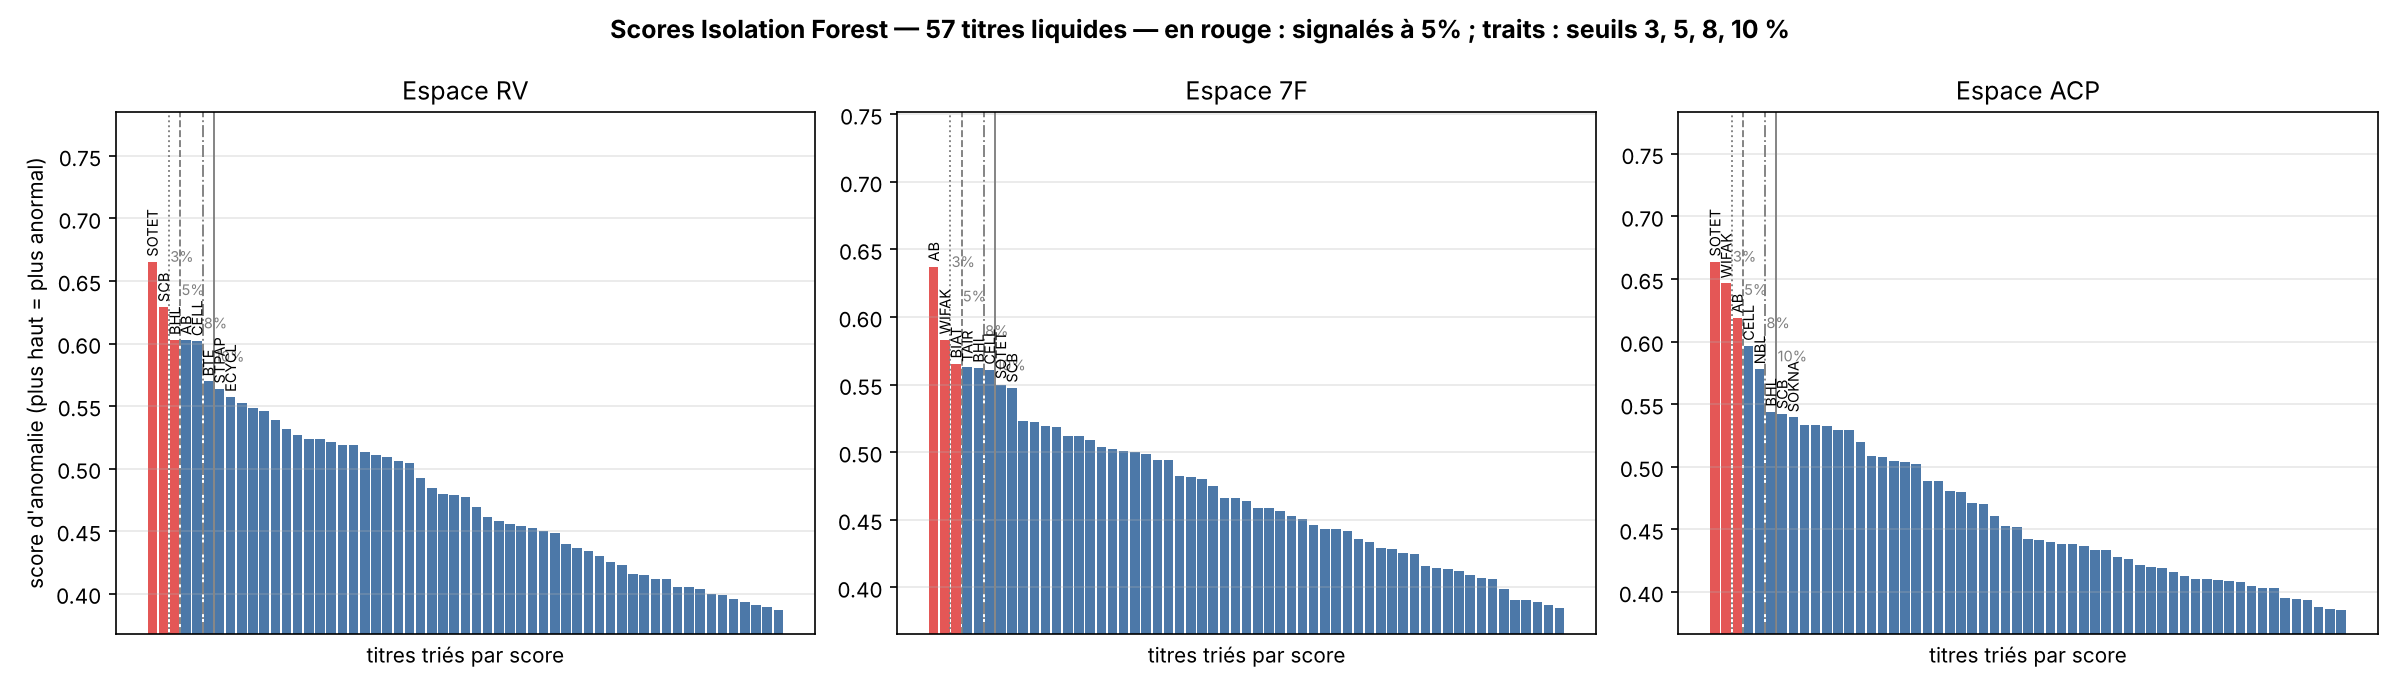
\includegraphics[width=\linewidth]{s4_scores_isolation_forest_liquides.png}
\caption{Scores Isolation Forest sur les 57 titres liquides.}
\end{figure}
\begin{figure}[H]\centering
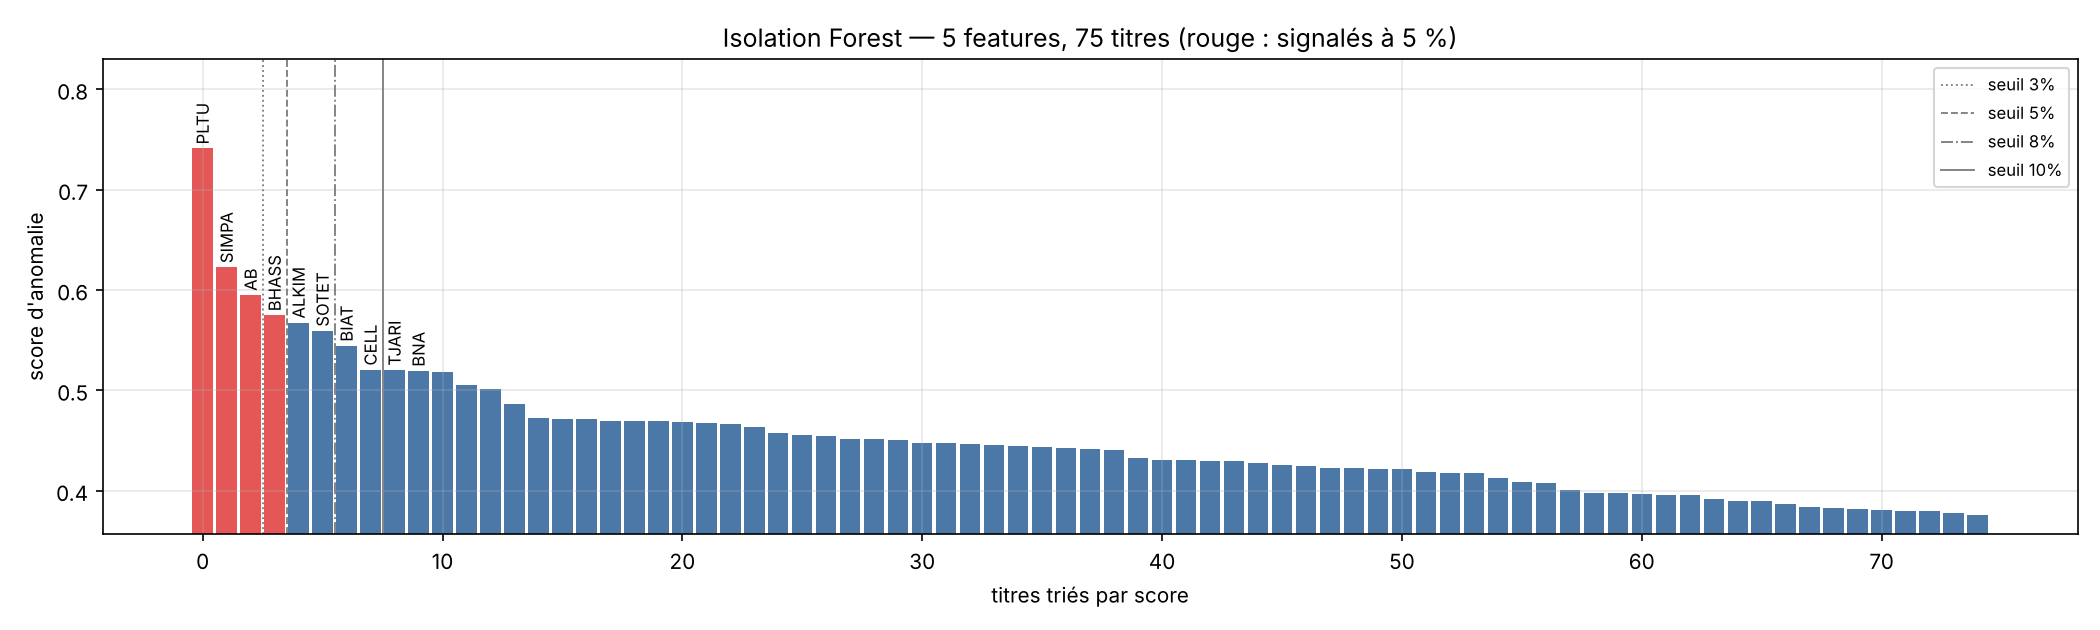
\includegraphics[width=0.9\linewidth]{s4b_scores_isolation_forest.png}
\caption{Scores Isolation Forest avec 5 features, 75 titres.}
\end{figure}

\section{Poids des portefeuilles de Markowitz}\label{ann:poids}
\begin{table}[H]\centering\small\caption{Poids des portefeuilles de Markowitz (75 titres, sans vente à découvert)}\label{tab:annexe-poids}
\begin{tabular}{lr@{\hspace{1.2cm}}lr@{\hspace{1.2cm}}lrr}\toprule
\multicolumn{4}{c}{Sharpe maximal (33 titres $>$ 0,1~\%)} & \multicolumn{3}{c}{Variance minimale (15 premiers)}\\ \cmidrule(r){1-4}\cmidrule(l){5-7}
Titre & Poids & Titre & Poids & Titre & $w \geq 0$ & forme fermée \\ \midrule
AB & 10{,}3~\% & CIL & 2{,}7~\% & PLTU & 36{,}9~\% & 36{,}8~\% \\
AL & 7{,}6~\% & ARTES & 1{,}7~\% & SIMPA & 14{,}3~\% & 14{,}5~\% \\
MGR & 7{,}0~\% & BHASS & 1{,}6~\% & BHASS & 3{,}3~\% & 3{,}4~\% \\
TINV & 6{,}8~\% & STIP & 1{,}4~\% & WIFAK & 2{,}7~\% & 2{,}7~\% \\
TJL & 5{,}9~\% & UBCI & 1{,}3~\% & AL & 1{,}8~\% & 1{,}9~\% \\
ATL & 5{,}7~\% & SOTUV & 1{,}2~\% & HL & 1{,}7~\% & 1{,}7~\% \\
TLS & 4{,}9~\% & ASSAD & 0{,}9~\% & SFBT & 1{,}6~\% & 1{,}8~\% \\
HL & 4{,}7~\% & STPIL & 0{,}9~\% & CC & 1{,}5~\% & 1{,}6~\% \\
SPDIT & 4{,}1~\% & TJARI & 0{,}8~\% & ALKIM & 1{,}5~\% & 1{,}5~\% \\
PGH & 3{,}7~\% & LNDOR & 0{,}7~\% & SPDIT & 1{,}5~\% & 1{,}6~\% \\
SOTET & 3{,}6~\% & TRE & 0{,}7~\% & SAH & 1{,}5~\% & 1{,}6~\% \\
AST & 3{,}6~\% & TPR & 0{,}5~\% & AST & 1{,}4~\% & 1{,}4~\% \\
STA & 3{,}6~\% & BNASS & 0{,}5~\% & UBCI & 1{,}3~\% & 1{,}4~\% \\
SAM & 3{,}5~\% & CITY & 0{,}4~\% & MGR & 1{,}3~\% & 1{,}3~\% \\
MPBS & 3{,}3~\% & MAG & 0{,}3~\% & TAIR & 1{,}2~\% & 1{,}2~\% \\
SMART & 3{,}1~\% & BL & 0{,}1~\% &  & &  \\
DH & 2{,}7~\% &  &  &  & &  \\
\bottomrule\end{tabular}\end{table}

\end{document}
